\documentclass[11pt]{article}
\usepackage[margin=1in]{geometry}
\usepackage{times}
\usepackage{setspace}
\setstretch{1.15}
\usepackage{graphicx}
\usepackage{booktabs}
\usepackage{amsmath}
\usepackage{amssymb}
\usepackage{caption}
\usepackage{xcolor}
\usepackage[colorlinks=true, linkcolor=blue!70!black, citecolor=blue!70!black, urlcolor=blue!70!black]{hyperref}
\urlstyle{same}
\renewcommand{\ttdefault}{cmtt}

% Adjust list spacing
\def\labelitemi{--}

\begin{document}

\begin{center}
    {\Large\bfseries Opening the Black Box of Large Language Models in Text-based Measurement: Staged Pipelines with Verifiable Checkpoints\par}
    \vspace{1em}
    {\normalsize\bfseries Milan Miric, Albert Roh, Nan Jia\par}
    \vspace{0.2em}
    {\small\itshape University of Southern California, Marshall School of Business\par}
    \vspace{0.8em}
    {\footnotesize\textbf{Proposal for Special Issue:} AI-Enabled Frontiers in Organizational Science (\textit{Organization Science})\par}
    \vspace{0.3em}
    {\footnotesize\textbf{Repository:} \url{https://github.com/HC-Geopolitics-Innovation/LLM-Text-Analysis-and-Synthesis}\par}
\end{center}

\vspace{1.5em}

\section{The Data Opportunity and Black-box Risk in LLM-based Measurement: A Staged Pipeline Approach}

Researchers increasingly use large language models (LLMs) to construct variables from text. The appeal is clear: long, noisy documents which have typically been unsuitable for processing with traditional techniques such as topic models or embeddings, such as 10-K filings and policy reports, can be processed by LLMs. This opens research contexts that were previously impractical to study at very large scale. However, when LLMs are used as an end-to-end solution---by providing a model with entire documents and asking it to return a numerical quantity---the LLM becomes a black box in that the final output is the only observable checkpoint. Researchers cannot see which parts of a document a measure rests on, what was omitted, or how judgments are made at intermediate stages. In addition, the outcome is sensitive to unobserved choices, making it difficult to reproduce.

This opacity creates three risks:
\begin{enumerate}
    \item \textbf{Validation.} Validating only the final output shows how often a measure is accurate in specific cases, but provides no systematic indication why it may have not been accurate. These aggregate measures can mask systematic errors: Carlson and Burbano (2026) show how these measures need to be validated by creating a heterogeneous set of approaches and then validating the outcomes on those approaches.
    \item \textbf{Reproducibility.} Rerunning an end-to-end process may not return the same measure when proprietary models are updated or retired; and because the process produces no intermediate outputs, other researchers cannot leverage the intermediate outputs generated by that process, and instead must re-create the entire effort.
    \item \textbf{Heterogeneity within documents.} An end-to-end measure collapses each document into a single output, concealing variation inside it. Researchers do not have control over which portion of a text document is driving the final outputs of the large language models, or whether for some parts of the model, the model is creating summaries and not processing these documents equally. Because these measures enter subsequent analyses as variables, the risk is not merely noisy measurement but biased analysis: when errors are systematic, a finding may reflect how a measure was produced rather than the phenomenon it is meant to capture. One might expect these risks to fade as models gain longer context windows and stronger reasoning. However, many of these concerns will remain. A more capable end-to-end model will only expose the final output, but the concerns will emerge from opacity and a lack of control over design choices, rather than from a limited capability.
\end{enumerate}

Recent work has acknowledged and begun to devise methodologies to overcome these risks. Carlson and Burbano (2026) propose a way of mitigating these concerns by systematic sensitivity analysis, including generating families of prompt variations, running them across models, and reporting the range of resulting downstream estimates. This approach reveals how much conclusions depend on implementation choices, but also focuses on a single albeit common task of textual classification. Processing long text documents and extracting specific insights nests a text classification choice within a black box of other data parsing, processing and synthesis functions. Using large language models for these other more complex textual analysis tasks creates more opportunities for the models to make choices. This is part of a broader literature which has emerged showing the idiosyncrasies of how these models can make individual choices, but when combined as part of a carefully crafted workflow can mimic at scale or improve what human workers would have achieved (Doshi et al., 2025; Dell'Acqua et al., 2026; Csaszar, Ketkar \& Kim, 2024). These studies have demonstrated important AI use in specific tasks, many of which could be easily integrated into an AI pipeline. However, the LLM processing of large information-rich text documents which could enable researchers to answer new and important questions requires finding a way to integrate and apply these methodologies as part of a pipeline which could in turn avoid introducing systematic noise and bias through black box algorithms.

Instead of using an end-to-end approach (e.g., using an LLM to parse, summarize, and extract a firm-specific score from text), we propose that researchers can use a staged pipeline that decomposes the process into verifiable steps, each generating a reusable and auditable intermediate output. In doing so, we show how this alleviates each of the three risks:
\begin{itemize}
    \item \textit{For validation}, intermediate outputs can be checked against ground-truth benchmarks at each stage, making it possible to locate where errors arise rather than only whether the final measure is noisy.
    \item \textit{For reproducibility}, a researcher who suspects that a prompt or model change affected a finding can vary one stage at a time and attribute any change in results to it.
    \item \textit{For heterogeneity}, intermediate outputs are retained for individual passages rather than whole documents, so aggregate measures can be traced back to their components and re-aggregated by contributor, section, or other conditions of interest.
\end{itemize}

Decomposing the process also allows each stage to use the tool best suited to it. LLMs excel at two types of tasks: (1) \textit{Synthesizing text}, that is, reading long, noisy passages and condensing them into short, information-dense outputs such as summaries or statements of position; and (2) \textit{Generating code}, that is, producing machine-readable instructions that can be systematically executed and tested. We use LLMs for synthesis and rely on established methods, such as embeddings and similarity measures, where they have proven routines, validation standards, and verifiable properties, applying them to condensed or sentence-level text rather than to whole documents. The pipeline thus combines the core strengths of LLMs with the known properties of established tools rather than replacing one with the other. Code generation also makes the pipeline easier to extend to other use cases: because the pipeline's code is available in a public repository, other researchers can use coding agents to adapt it to their own data and questions (Appendix D).

We demonstrate the application of this approach in a setting relevant for organization researchers: how congressional debate over regulating a technology relates to changes in the innovation trajectories of firms exposed to it. Studying this question requires understanding and quantifying the nature of the policy debate which exists and how it might be leveraged by researchers. This also requires measuring the extent to which the issues being discussed in the debate represent threats or opportunities for firms.

We focus on the policy debate over user data privacy that emerged in the mid-2010s related to technology companies collecting customer data, the Cambridge Analytica scandal related to the use of Facebook data by third-party companies, and document the relationship between the debate of policymakers which coincided with shifts in the innovation policy of firms. Studying this question requires identifying which firms were likely impacted by this debate, so they can be compared with firms that credibly were not. That information is embedded in two kinds of long, noisy documents: congressional hearing transcripts, which average roughly 40,000 words and alternate between testimony and questioning from many participants, and firms' 10-K filings. The setting puts all three risks at stake: because the exposure measure assigns firms to treatment and control groups, systematic error in it would bias the estimated effect; because other researchers may want to extend the measure to studying other policies, it must be reproducible in parts; and because a committee's stance may reflect its members broadly or only a few vocal participants, heterogeneity within hearings matters for interpretation.

\section{Our Framework: A Staged Pipeline for LLM-based Measurement}

We develop a framework that illustrates how LLMs can be used within a data pipeline without ceding full control to them. After data preparation, the pipeline proceeds through three stages (text summarization, stance extraction, and relevance to firms' business areas), each composed of discrete steps that produce intermediate outputs. Each output can be validated, reused, and disaggregated, addressing the three risks above. Researchers can adapt these stages to extract different insights or apply them to data of their choice.

\subsection{Overview of Data Pipeline and Processing Stages}

\begin{itemize}
    \item \textbf{Stage 1: Data Preparation:} Assembling and structuring the corpora before any LLM is applied. We parse congressional hearing transcripts from the U.S. Government Publishing Office into speaker-attributed turns, extract business descriptions (Item 1) from S\&P 500 firms' 10-K filings, and retrieve independent C-SPAN hearing abstracts as a validation benchmark. Defects such as undigitized transcripts are flagged rather than dropped, so every exclusion can be inspected.
    \item \textbf{Stage 2: Text Summarization:} Taking large, complex textual documents that contain considerable noise alongside embedded data, partitioning them into chunks, and using LLMs to generate, synthesize, and aggregate textual summaries. We demonstrate this approach on congressional hearing transcripts (see Appendix B for data sources and processing), summarizing long and convoluted documents into concise summaries that can subsequently be used for text classification, topic modeling, or semantic distance estimation in more reliable ways.
    \item \textbf{Stage 3: Stance Extraction:} Using LLMs to identify the positions of different actors (e.g., members of Congress, firms, government agencies) on specific topics, allowing researchers to distill the nuances of arguments and positions that each individual takes on an issue. We apply this to congressional hearings to identify the stances of members of Congress on key issues, classified as support, concern, or neutral, in a format that can be utilized in subsequent research.
    \item \textbf{Stage 4: Debate Relevance to Firm Business Areas:} Using the distilled stances of individuals within the debate, we create a synthesis of the policy debate. This synthesis, or an embedding of the underlying statements, can then be compared to the business descriptions of firms to identify which firms are exposed to the debate. In our empirical context, this means framing the key issues that policymakers are debating and attempting to regulate. We then compare this to the business descriptions (Item 1) in firms' 10-K filings. This allows us to identify and study firms that are exposed to the debate versus those that are not.
\end{itemize}

\subsection{Adapting the Pipeline for Other Research Questions}

Because each stage is modular and its code is available in our repository, researchers can reuse the pipeline in part or in full. For example, they can apply the same stages to hearings of other committees or to other policy topics, or replace the stance-extraction stage to measure a different construct while keeping data preparation and summarization fixed.

Furthermore, LLMs' ability to generate code lowers the cost of such adaptation: these models also excel at writing code that is automatically tested, verified, and validated. By providing our pipeline's code and methodologies in a GitHub repository where the codebase is available, researchers can use their own coding agents to either improve upon our methodology or apply this methodology to their own setting and data.

\section{Current Status of Project}

We have currently developed a research pipeline, focused on the specific question outlined above: the relationship between congressional debate about user data privacy and the innovation trajectory of technology companies, made available on the associated GitHub repository for this project. This pipeline demonstrates the transformation from raw transcripts of congressional hearings to a series of research outputs: textual summaries, summaries of perceived priorities (support/concerns identified by policymakers), and an index for policy relevance for publicly listed firms. This is a prototype of what can be done (using one set of approaches and design choices in the LLM pipeline). However, as we aim to show, and much like we are advocating, this pipeline can be verified, adopted, or adapted to other projects and applications.

\subsection{Expected Deliverables}

\begin{itemize}
    \item \textbf{Reproducible LLM Data Pipeline for Text Summarization, Stance Extraction, and Topic Relevance}
    \item \textbf{Public Datasets for Subsequent Research:} From the data of 36K Congressional Hearings from 1995--2025 (currently 2,352 hearings for the House and Senate Science Committees): full chunked text, intermediate summaries, list of topics discussed, summarized stances, an index of committee stances on topics discussed in hearings, and an index of relevance of those topics for publicly listed firms based on Item 1 business descriptions (1995--2025).
    \item \textbf{Illustrative Empirical Results:} Demonstration of the empirical results of the privacy regulation applied to investigate the impact of privacy regulation on the trajectory of corporate innovation.
    \item \textbf{Instructions and Framework for Deployment for Follow-on Research}
\end{itemize}

\subsection{Datasets (Outputs from Focal Research Project)}

\begin{itemize}
    \item \textbf{Text Summaries for Congressional Testimony from 1995 to 2025:} Cleaned and chunked testimony, summarized testimony chunks, finalized text summaries.
    \item \textbf{Index of Committee Stances in Congressional Debate:} Topics within congressional debate, filtered chunks focused with a stance on a focal topic, summarized positions on a focal topic, and an aggregated index of committee stances on topics discussed.
    \item \textbf{Index of Relevance of Congressional Debate for Publicly Listed Firms:} Summarized congressional stances and company business descriptions based on 10-K filings, relevance index for individual company filings and congressional topic stances, and an aggregated index for topical relevance.
\end{itemize}

\subsection{Example of Empirical Application}

\begin{itemize}
    \item \textbf{Demonstration of the Policy Relevance Index:} Demonstrating the use of the constructed policy relevance index regarding the impact of congressional debate on the innovative trajectories of publicly listed firms. Using the context of the Cambridge Analytica scandal, we demonstrate how these tools can be used to identify firms that were in treated or control groups, allowing for an event study design to examine changes in innovation trajectories following these events.
\end{itemize}

\subsection{Key Risks and Limitations in Implementation}

We have tested the viability of our empirical strategy and have developed a working prototype of its deployment. We have confidence that this methodology will provide useful outputs. We have a goal of demonstrating this with as large a dataset as possible (the population of congressional testimony, public firm 10-Ks, and major policy topics discussed). We also recognize the potential for different ways of constructing and aggregating data. Because each of these approaches is time-consuming, we are committed to implementing all of them, but may become constrained in the number of individual specifications we can add.

\section{How This Advances Organizational and Social Science}

Long-form documents such as congressional hearings, regulatory filings, and corporate disclosures record how organizations and governments deliberate, yet they have been difficult to use: established text methods work best on short, information-dense text, and end-to-end LLM use relaxes this constraint only by introducing opacity. Our approach relaxes this constraint while alleviating the opacity of end-to-end use. If successful, it advances organizational research in three ways:

First, it provides a pipeline that turns long, noisy documents into measures whose construction can be inspected stage by stage. LLM-based measures thus become auditable research objects rather than outputs taken on trust, and the pipeline offers a template for reporting them, including intermediate outputs, stage-level validation, and stage-specific sensitivity analysis.

Second, it provides a public research dataset: summaries of more than 2,300 congressional hearings, a panel of legislators' stances by topic, and firm-level measures of exposure to policy debate. Because intermediate outputs are released alongside the final measures, other researchers can build on any stage, for example by re-aggregating stances by member or relating firm exposure to new outcomes.

Third, the framework enables a new form of replication. Because the pipeline is shared as a modular repository, researchers can direct coding agents to rebuild or adapt it at low cost. And because each stage produces outputs that can be compared with ours, a replication need not succeed or fail as a whole: discrepancies can be located at the stage where they arise. Replication thus shifts from an all-or-nothing comparison of final results to a stage-by-stage check.

Together, these contributions allow researchers both to do existing work better and to do new work. Existing work improves because the risks identified above become testable: when each stage is validated, systematic error can be detected and located before it biases a finding, and when a replication can localize discrepancies, disagreements over results can be traced to specific choices rather than left unresolved. New work becomes possible because researchers no longer face a choice between avoiding long-form documents and relying on measures that cannot be checked. Hearings, regulatory proceedings, and corporate disclosures, which record how organizations and governments deliberate, can support credible measures at scale; and because outputs are retained within documents, researchers can ask not only what a collective position is but who shapes it. The aim is not more research from the same materials, but better research from materials previously out of reach.

\vspace{2em}
\section*{References}
\begin{itemize}
    \item Carlson, N., \& Burbano, V. (2026). Validating Large Language Models in Text Analysis: A Sensitivity Framework. \textit{Working Paper}.
    \item Csaszar, F. A., Ketkar, S., \& Kim, M. (2024). Artificial intelligence and organizational decision making. \textit{Academy of Management Annals}.
    \item Dell'Acqua, F., McFowland, E., Mollick, E. R., Lifshitz-Assaf, H., Kellogg, K., Rajendran, S., Krayer, L., Candelon, F., \& Lakhani, K. R. (2026). Navigating the Jagged Technological Frontier: Field Experimental Evidence of the Effects of AI on Knowledge Worker Productivity and Quality. \textit{Management Science}.
    \item Doshi, A. R., Bell, J. J., Mirzayev, E., \& Vanneste, B. S. (2025). Generative artificial intelligence and evaluating strategic decisions. \textit{Strategic Management Journal}, 46(3), 583--610.
    \item Kogan, L., Papanikolaou, D., Seru, A., \& Stoffman, N. (2017). Technological Innovation, Resource Allocation, and Growth. \textit{Quarterly Journal of Economics}, 132(2), 665--712.
\end{itemize}


\clearpage
\appendix

\begin{center}
    {\Large\bfseries Online Appendices: Opening the Black Box of Large Language Models in Text-based Measurement\par}
    \vspace{0.5em}
    {\large\itshape Staged Pipelines with Verifiable Checkpoints\par}
    \vspace{1em}
    {\normalsize\bfseries Milan Miric, Albert Roh, Nan Jia\par}
    \vspace{0.2em}
    {\small\itshape University of Southern California, Marshall School of Business\par}
    \vspace{0.8em}
    {\footnotesize\textbf{Proposal for Special Issue:} AI-Enabled Frontiers in Organizational Science (\textit{Organization Science})\par}
    \vspace{0.3em}
    {\footnotesize\textbf{Repository:} \url{https://github.com/HC-Geopolitics-Innovation/LLM-Text-Analysis-and-Synthesis}\par}
\end{center}

\vspace{1.5em}

\section*{Appendix A. Overview of Steps in Large Language Model Enabled Research Pipeline}
\addcontentsline{toc}{section}{Appendix A. Overview of Steps in Large Language Model Enabled Research Pipeline}

\subsection*{A.1. Long-Document Text Summarization}
\subsubsection*{A.1.1. Overview of Processing Pipeline}

Processing long text documents is a challenge for large language models because they are prone to degradation in attention as input text increases (Liu et al., 2023), struggle to preserve factual detail across multiple conversational turns, and can introduce hallucinations during complex open-ended synthesis. 

To overcome these constraints, we propose a staged Map-Reduce summarization pipeline that preserves document integrity:
\begin{enumerate}
    \item \textbf{Data Ingestion \& Speaker Turn Partitioning:} Documents are ingested from source XML/HTML formats, parsed into turn-level records, and attributed to specific speakers.
    \item \textbf{Chunk-Level Map Summarization:} Documents exceeding the model's high-attention context threshold are divided into sequential semantic chunks (roughly 4,000--8,000 tokens) with overlapping boundaries to prevent conversational clipping. Prompts focus the model on identifying substantive factual points.
    \item \textbf{Hierarchical Reduce Synthesis:} Intermediate chunk summaries are aggregated through a structured reduce prompt that reconciles cross-chunk themes into an entity-attributed document summary.
    \item \textbf{Discriminant Validity Checkpoint:} Summaries are validated against external human benchmarks (such as professional C-SPAN editorial abstracts).
\end{enumerate}

\subsubsection*{A.1.2. Application: Summarizing Long Text Congressional Hearings}

We apply this architecture to 2,352 congressional committee hearings before the House Science, Space, and Technology Committee and the Senate Commerce, Science, and Transportation Committee. Transcripts average roughly 40,000 words. Figure 1 reports the cosine similarity between our generated summaries and independent, professional C-SPAN abstracts across same-hearing, same-committee, and different-committee pairs.

\begin{figure}[htbp]
    \centering
    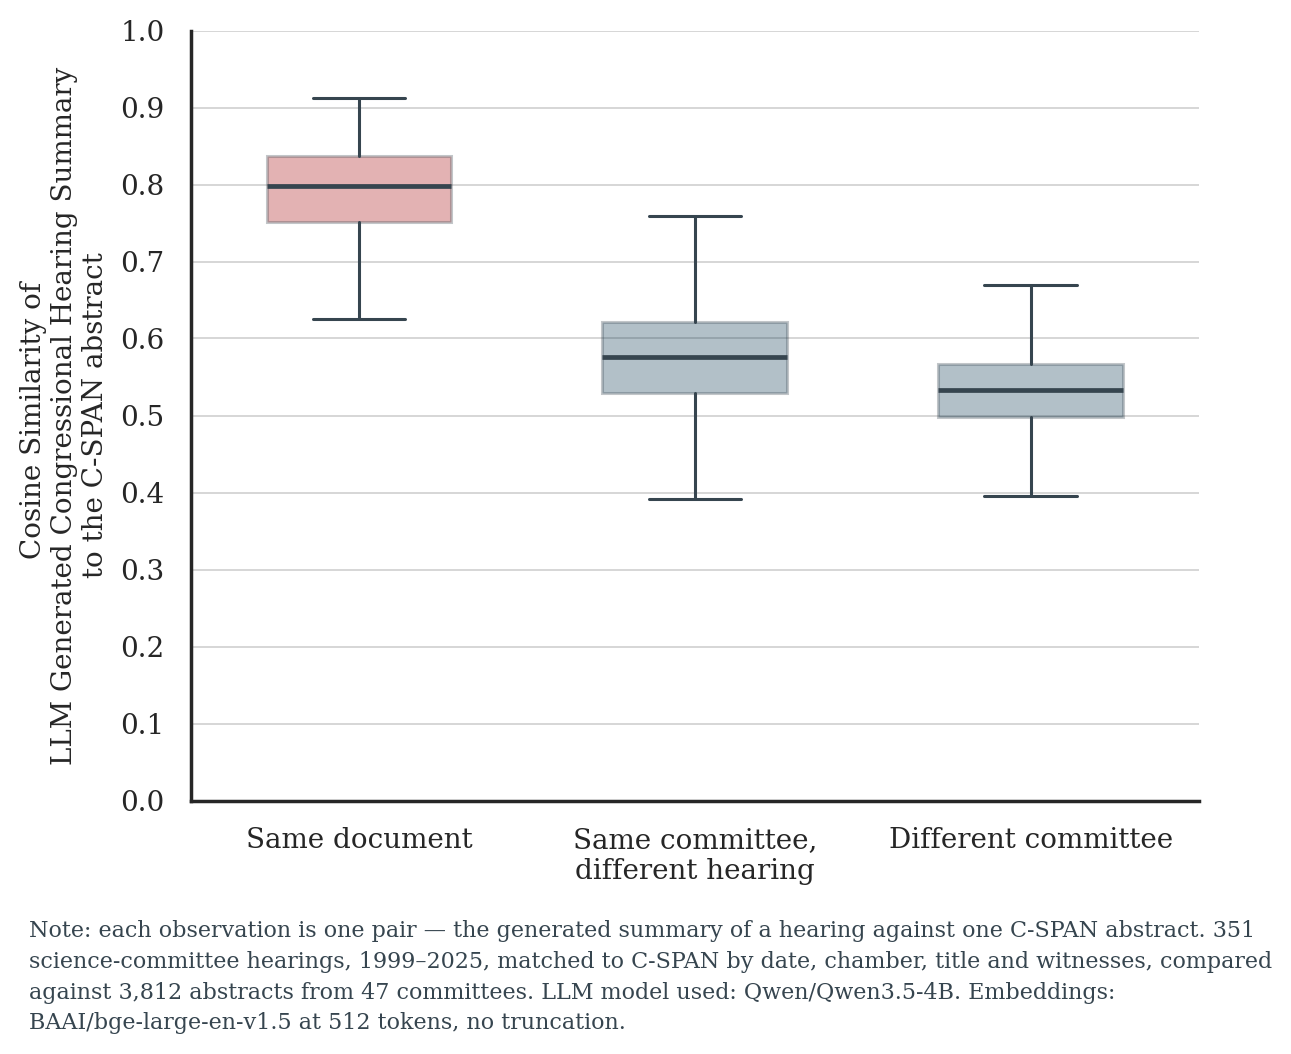
\includegraphics[width=0.85\textwidth]{figures/fig1_cosine_similarity.png}
    \caption{\textbf{Cosine Similarity Between Hand-Coded Summaries and Large Language Model Summaries across Committees.}}
    \vspace{4pt}
    {\footnotesize\textit{Notes: Comparison of cosine similarity distributions between model-generated summaries and independent human-authored C-SPAN abstracts. Same-document pairs exhibit high semantic alignment, whereas different-committee pairs show distinct separation, verifying discriminant validity.}\par}
\end{figure}

\subsubsection*{A.1.3. Research Outputs}

\begin{itemize}
    \item \textbf{Cleaned Transcript Segments:} Fully segmented, speaker-attributed transcripts with timestamp and witness provenance.
    \item \textbf{Intermediate Chunk Summaries:} Auditable, passage-level summaries supporting localized verification.
    \item \textbf{Final Hearing Summaries:} Entity-attributed committee hearing summaries for downstream classification.
\end{itemize}

\subsection*{A.2. Extracting Topics, Positions, and Arguments from Long-Form Documents}
\subsubsection*{A.2.1. Overview of Processing Pipeline}

\begin{enumerate}
    \item \textbf{Taxonomic Clustering \& Codebook Generation:} We use LLMs to extract emerging policy topics from statements and crosswalk them to standardized classification systems like the Comparative Agendas Project (CAP).
    \item \textbf{Stance Extraction:} Identifying discrete positions (support, concern, neutral) held by individual speakers on focal topics.
    \item \textbf{Validation Against External Criteria:} Agreement audits across prompt variants and cross-validation against legislative roll-call voting records.
\end{enumerate}

\subsubsection*{A.2.2. Application: Extracting Stances and Arguments around Focal Topics}

Figure 2 illustrates the distribution of identified congressional stances across major technological domains, highlighting the balance of support versus concern.

\begin{figure}[htbp]
    \centering
    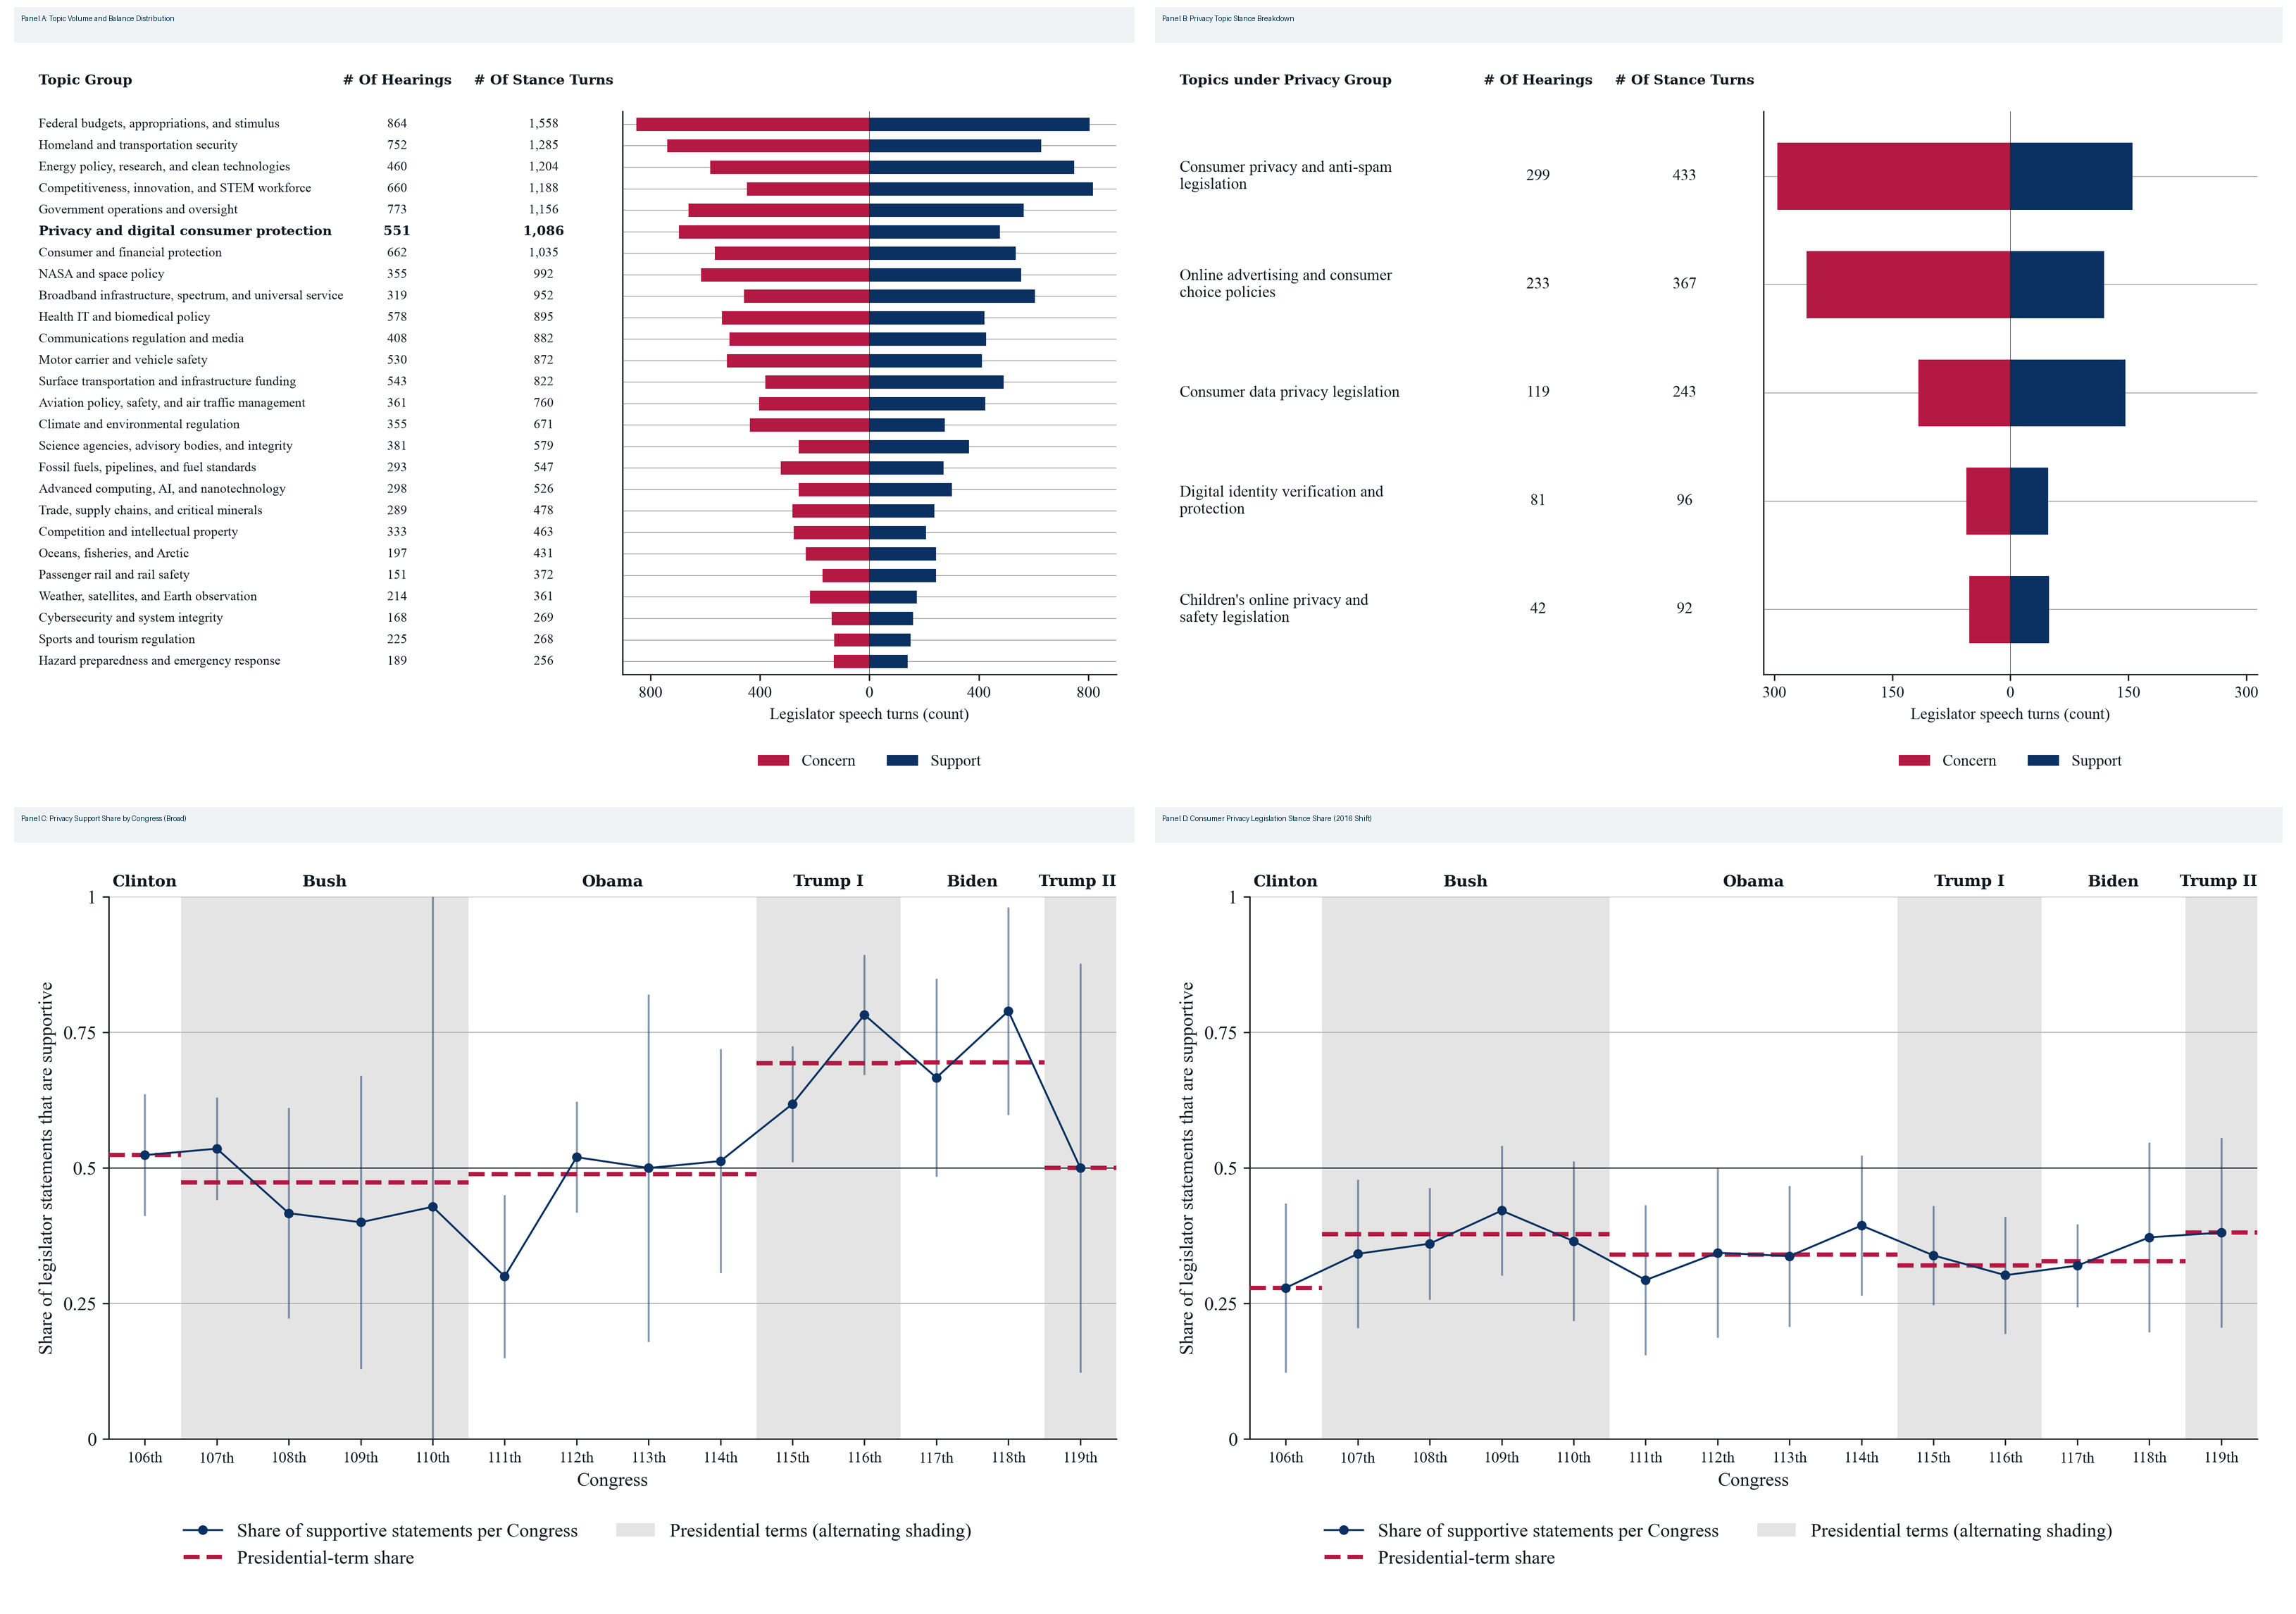
\includegraphics[width=0.90\textwidth]{figures/fig2_topics_stances_4panel.png}
    \caption{\textbf{Topics and Overview of Stance (Support / Concern of Policymakers).}}
    \vspace{4pt}
    {\footnotesize\textit{Notes: Four-panel overview tracking congressional topic prevalence, stance distributions, member polarization, and longitudinal legislative attention across science and technology hearings.}\par}
\end{figure}

\subsubsection*{A.2.3. Research Outputs}

\begin{itemize}
    \item \textbf{Standardized 111-Topic Policy Codebook:} Fully crosswalked to CAP categories.
    \item \textbf{Member-Topic Stance Panel:} Micro-level dataset tracking individual member arguments and policy positions over time.
\end{itemize}

\subsection*{A.3. Policy Relevance for Publicly Listed Firms}
\subsubsection*{A.3.1. Overview of Processing Pipeline}

\begin{enumerate}
    \item \textbf{Corporate Text Extraction:} We extract Item 1 (Business Description) from annual 10-K filings.
    \item \textbf{Centroid Embedding Estimation:} Generating high-dimensional dense embeddings of policy debate stances and firm business summaries.
    \item \textbf{Cosine Distance Scoring:} Measuring semantic cosine similarity between each firm's business profile and the policy centroid, demeaned relative to sample benchmarks.
\end{enumerate}

\subsubsection*{A.3.2. Application: Connecting Focal Concerns and Opportunities of Policymakers to Business Areas of Publicly Listed Firms}

Figure 3 reports topic relevance scores for publicly listed firms regarding Consumer Data Privacy Legislation (Topic 68). Panel A reports industry-level exposure by NAICS sector relative to the sample mean. Panel B reports firm-level relevance scores for selected high- and low-relevance firms.

\begin{figure}[htbp]
    \centering
    \begin{minipage}{0.48\textwidth}
        \centering
        \textbf{\footnotesize Panel A: NAICS Sector Cosine Relative to Mean}\par\vspace{2pt}
        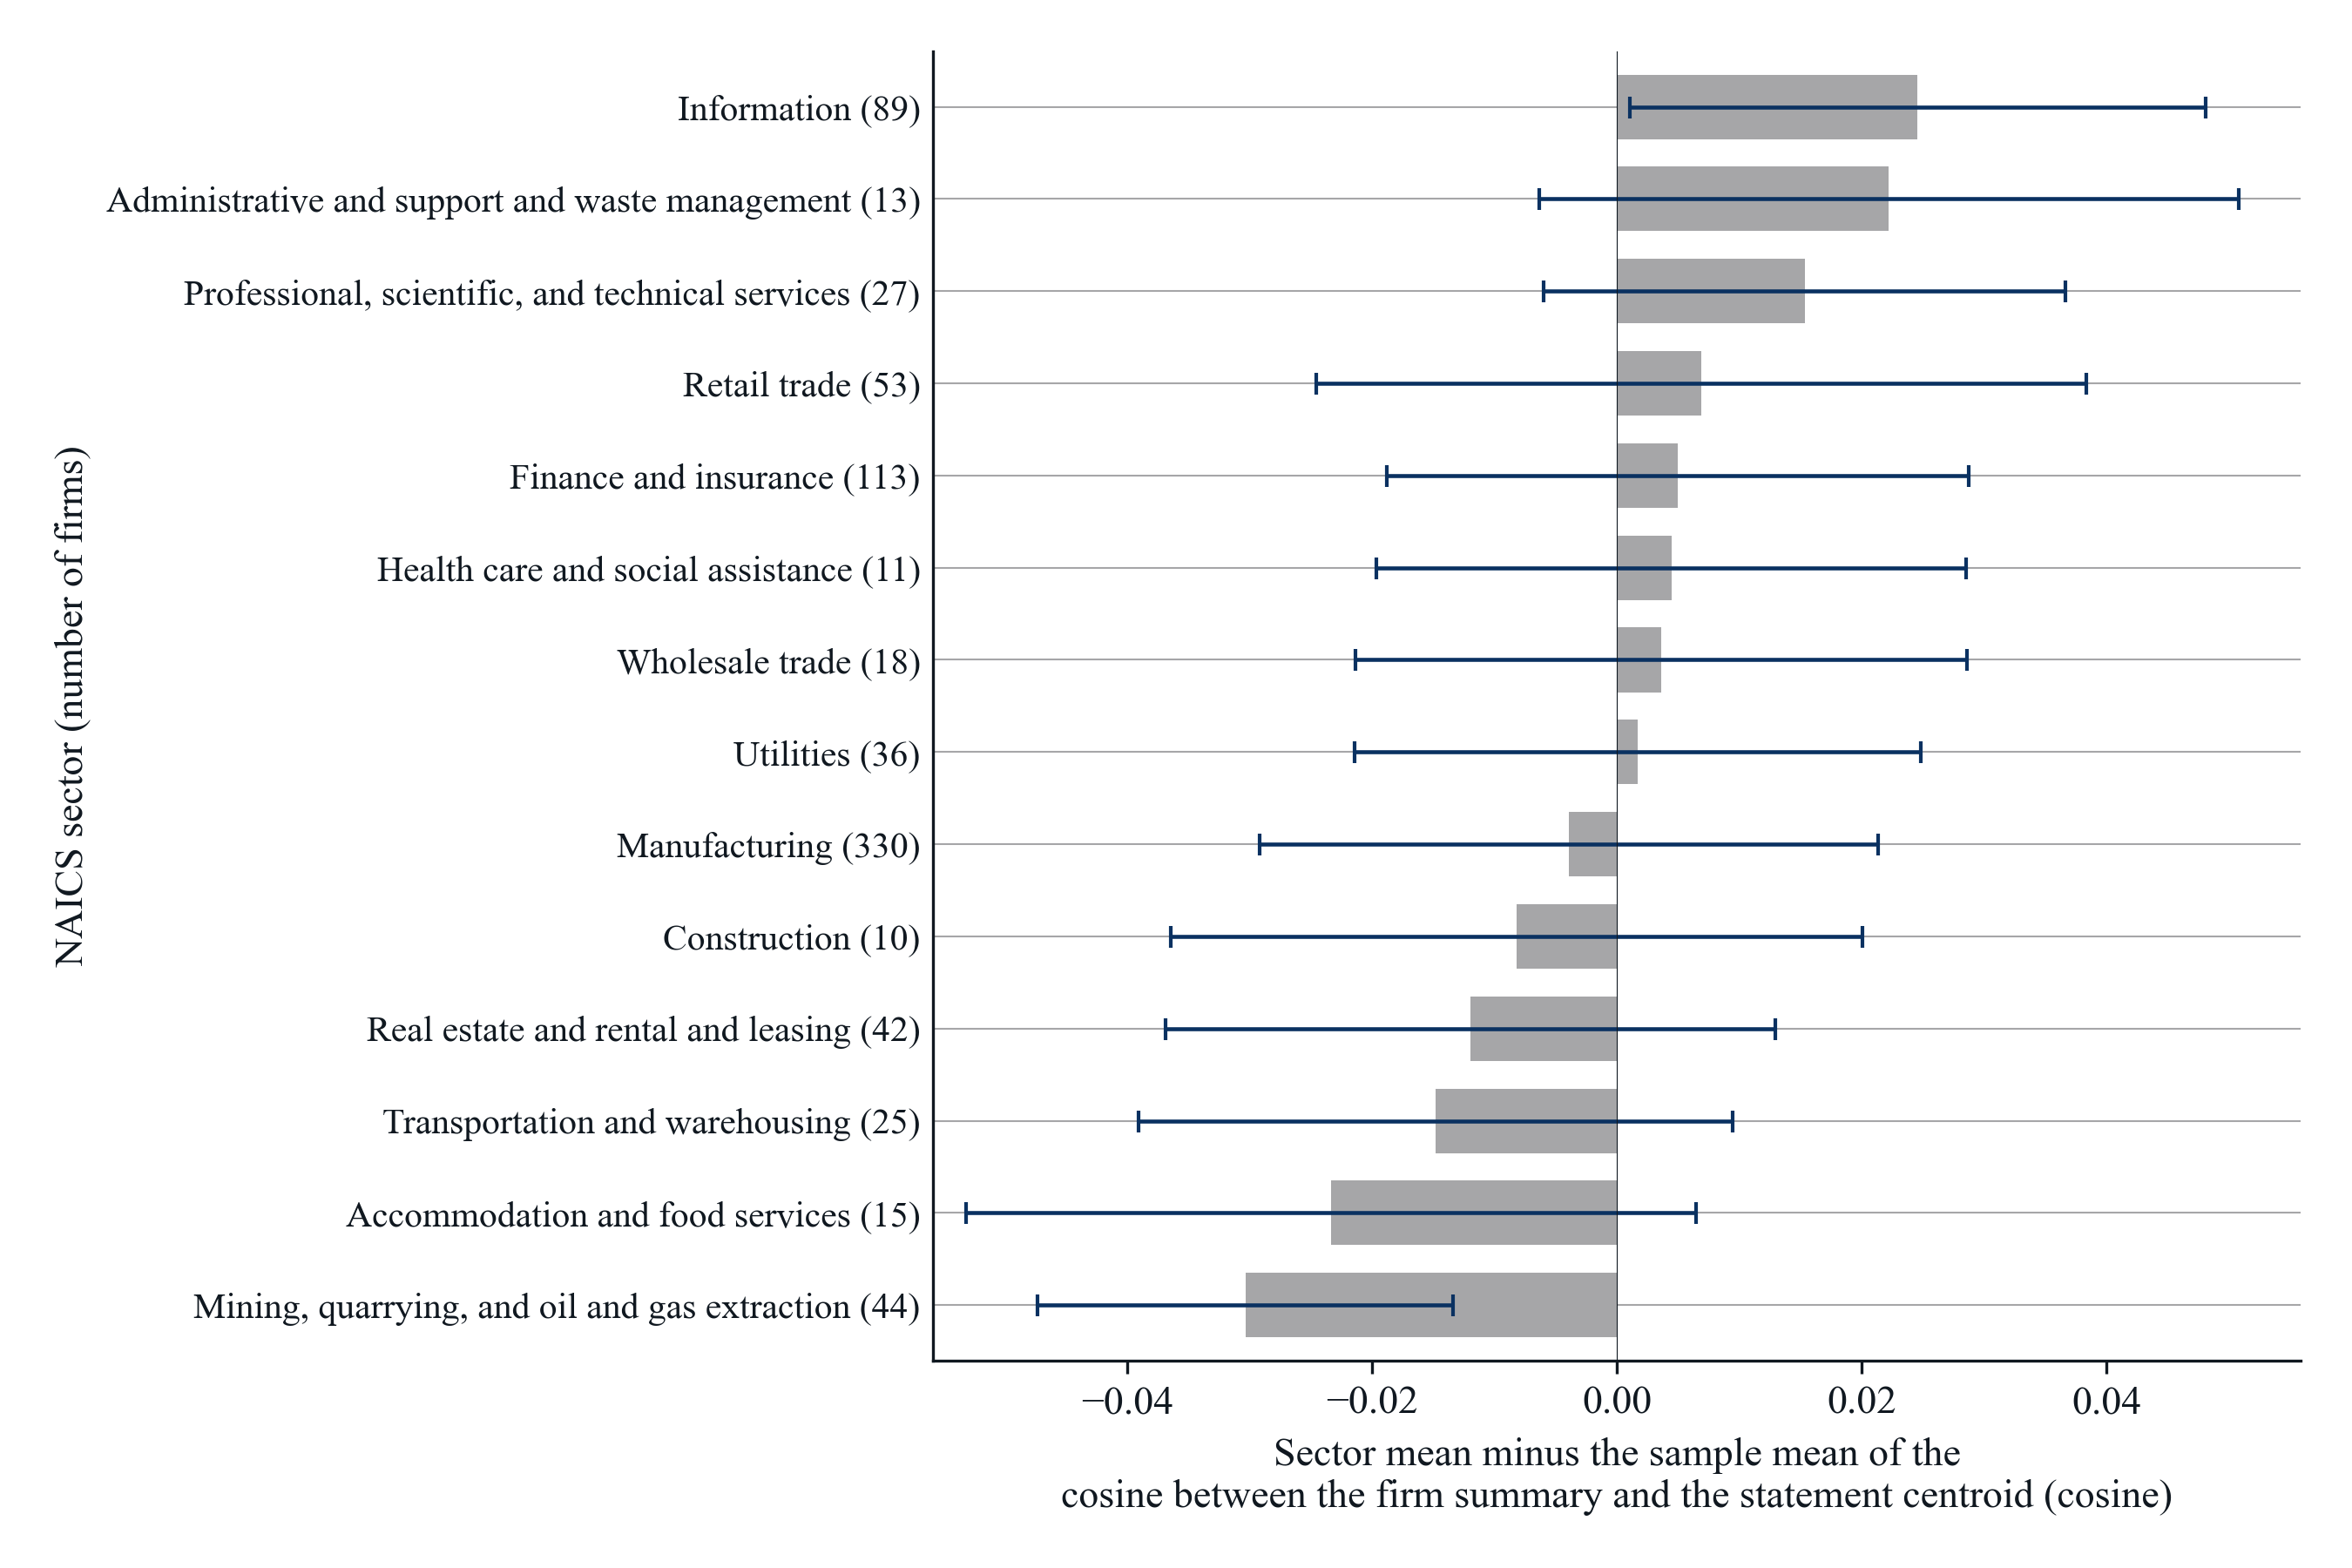
\includegraphics[width=\textwidth]{figures/fig3_panel_a_naics_relevance.png}
    \end{minipage}\hfill
    \begin{minipage}{0.48\textwidth}
        \centering
        \textbf{\footnotesize Panel B: Selected High and Low Relevance Firms}\par\vspace{2pt}
        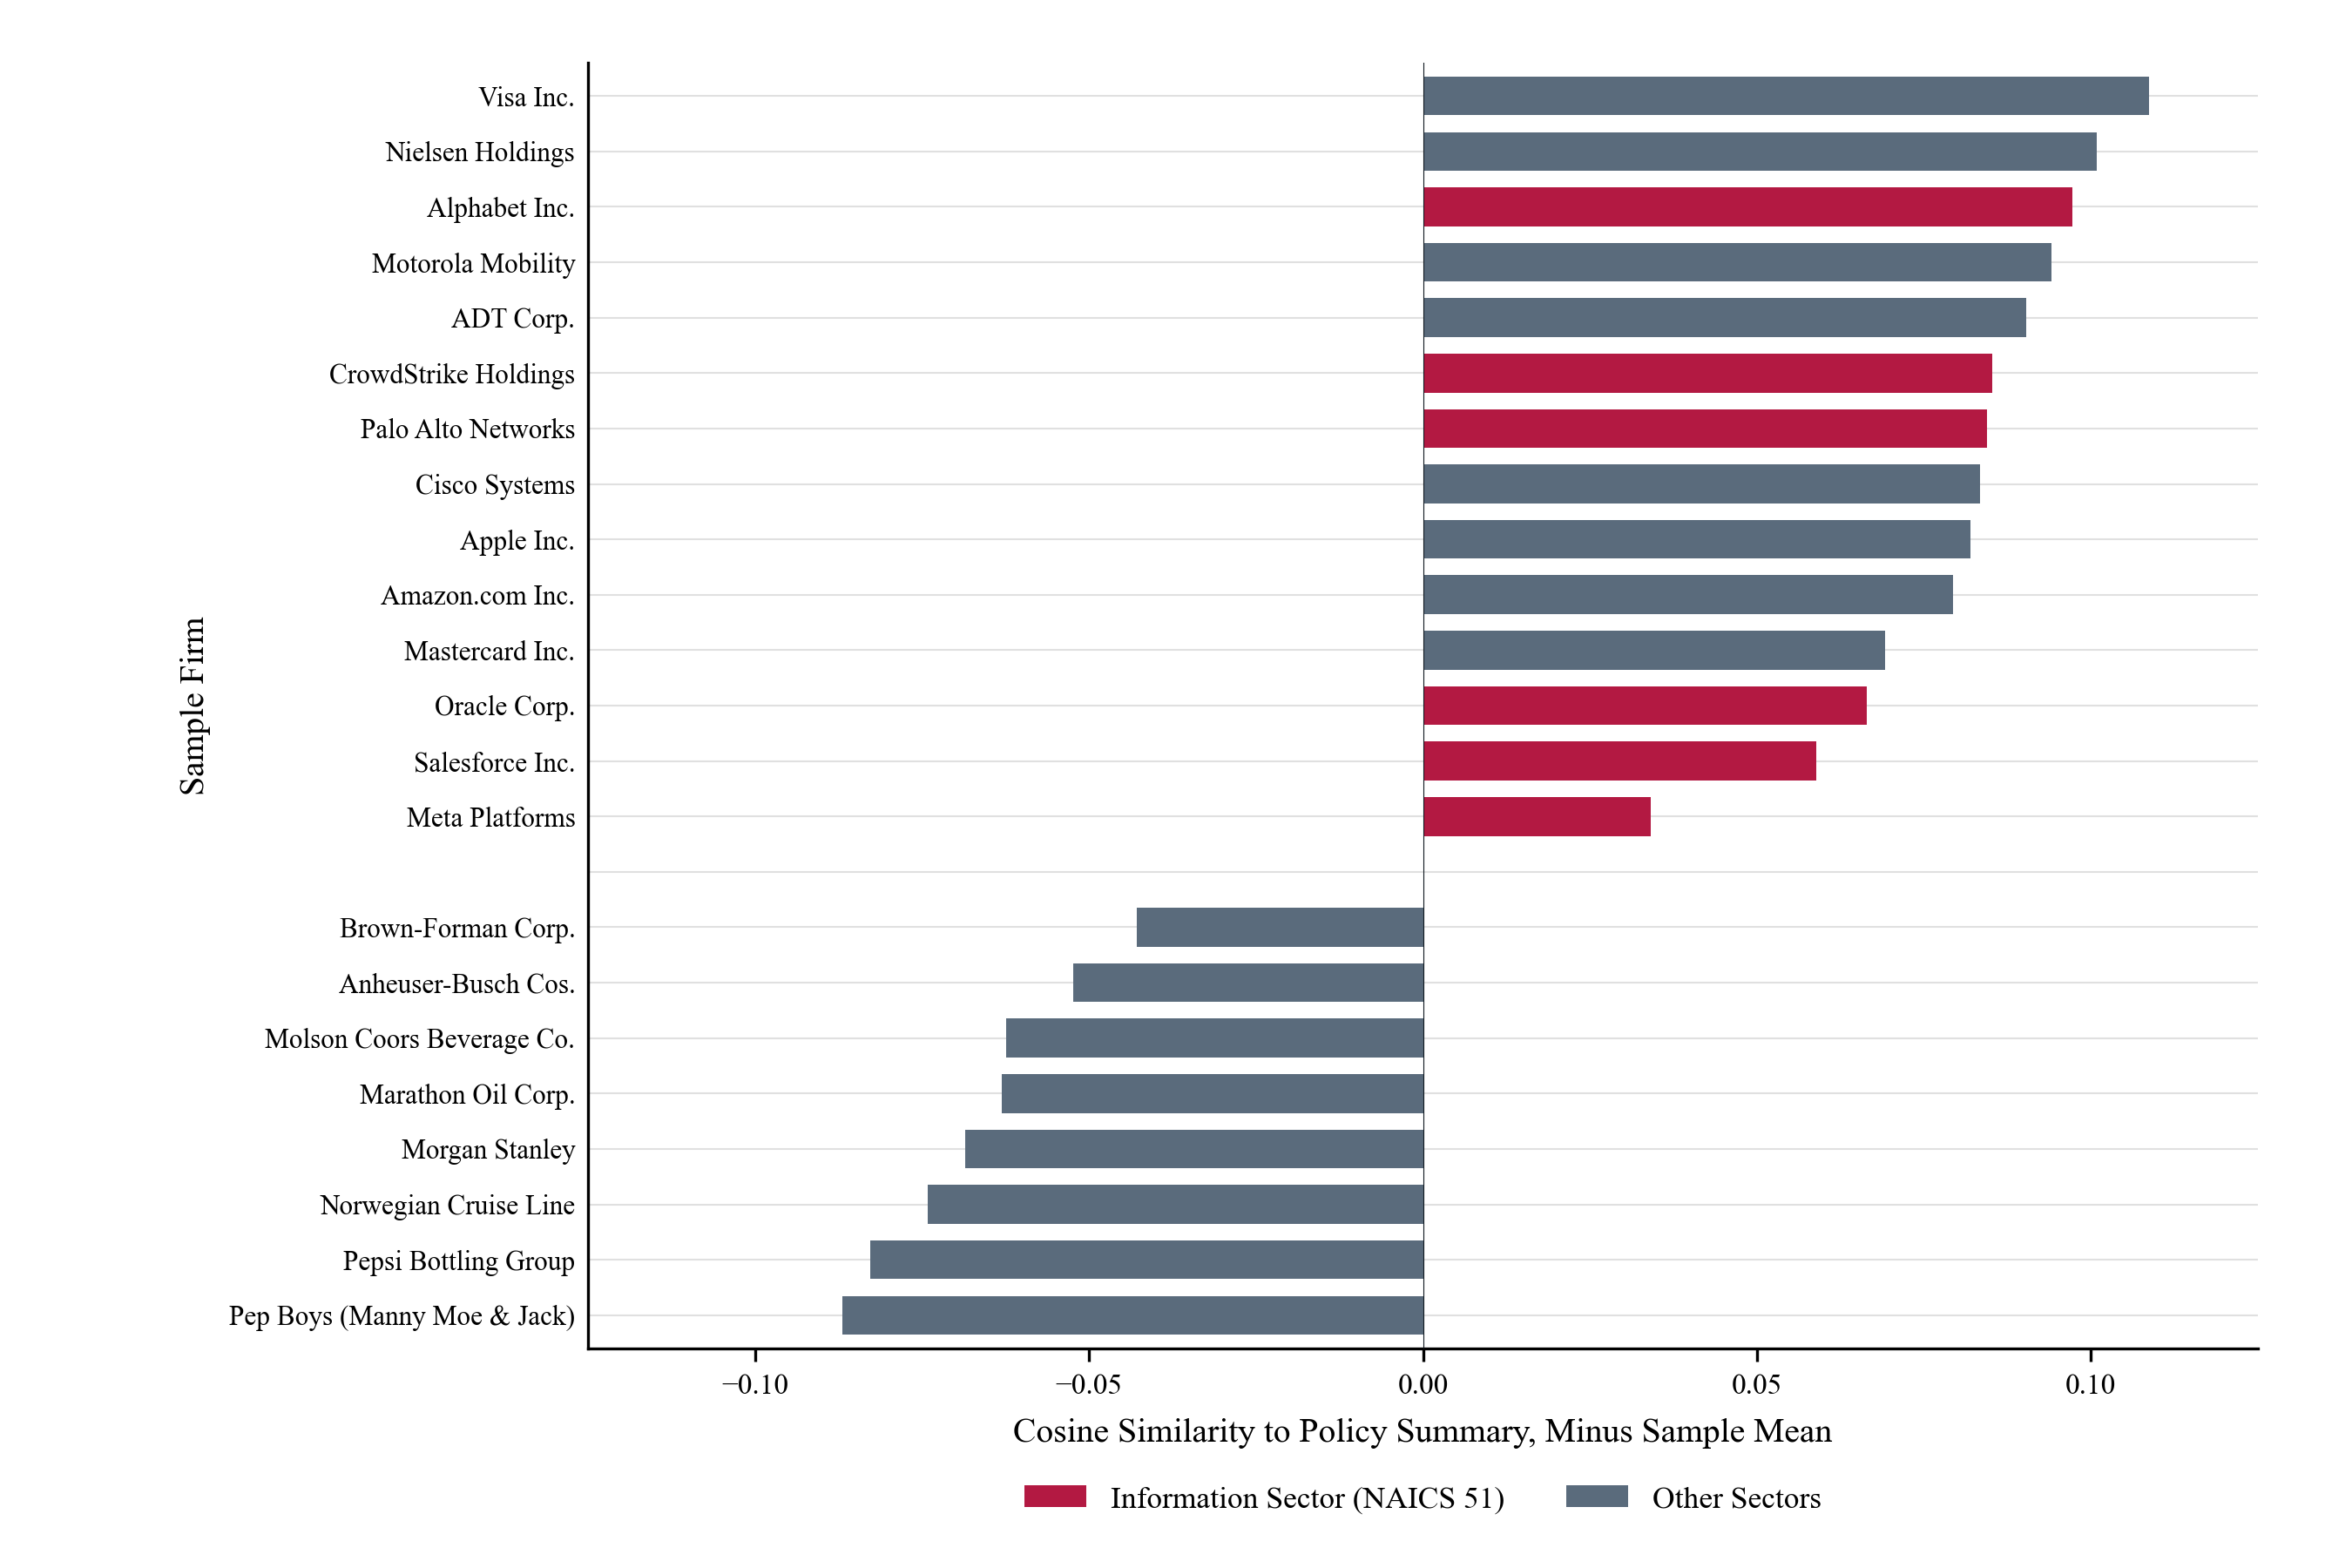
\includegraphics[width=\textwidth]{figures/fig3_panel_b_top_firms.png}
    \end{minipage}
    \caption{\textbf{Topic Relevance Scores for Publicly Listed Firms.}}
    \vspace{4pt}
    {\footnotesize\textit{Notes: Panel A reports firm summary cosine similarity by NAICS sector relative to the sample mean (Topic 68 policy summary vector). Panel B reports demeaned topic relevance scores for selected high- and low-relevance firms, color-coded by sector (Information sector in crimson, other sectors in slate grey). Both panels share identical aspect ratios ($1.5$).}\par}
\end{figure}

\subsubsection*{A.3.3. Research Outputs}

\begin{itemize}
    \item \textbf{10-K Item 1 Business Description Corpus:} Curated and verified annual report summaries.
    \item \textbf{Firm-Topic Relevance Panel:} Longitudinal exposure scores linking public firms to policy debates.
\end{itemize}

\newpage
\section*{Appendix B. Overview of Datasets Used for Data Pipeline}
\addcontentsline{toc}{section}{Appendix B. Overview of Datasets Used for Data Pipeline}

This appendix provides an integrated overview of the primary input corpora, verification benchmarks, and research output datasets utilized across our AI-enabled pipeline.

\subsection*{A. Primary Data Inputs}
\begin{itemize}
    \item \textbf{Congressional Hearings Dataset (U.S. GPO GovInfo CHRG Collection):} Complete package manifest of 36,378 hearings spanning 1995--2025. Focal sample covers 2,352 hearings before House Science and Senate Commerce committees containing 93.6 million words across 116,000 speaker turns.
    \item \textbf{Publicly Listed Firms Business Descriptions (SEC Form 10-K Filings):} Full SEC EDGAR archive accessed via sec-api.io, comprising 305,140 annual reports. Mapped to financial fundamentals through a bijective CRSP--Compustat crosswalk linking 25,207 CIK $\leftrightarrow$ GVKEY identifier pairs. Yields 22,299 S\&P 500 reports complete with extracted text and usability flags.
\end{itemize}

\subsection*{B. Verification Data}
\begin{itemize}
    \item \textbf{Independent Reference Abstracts (C-SPAN Archives API):} 18,697 committee program summaries covering 1995--2025 written by professional C-SPAN editors independently of congressional staff, serving as an external ground-truth benchmark for discriminant validity testing.
\end{itemize}

\subsection*{C. Output Research Datasets}
\begin{itemize}
    \item \textbf{Text Summarization Corpus (Stage 2 Outputs):} Cleaned, turn-attributed transcripts; intermediate chunk summaries; finalized hearing summaries (\texttt{hearing\_summaries.parquet}).
    \item \textbf{Policy Stance Panel Dataset (Stage 3 Outputs):} Standardized 111-topic policy taxonomy codebook (\texttt{frozen\_codebook\_111.parquet}); longitudinal member-topic stance panel (\texttt{member\_stance\_panel.parquet}).
    \item \textbf{Corporate Topic Relevance Dataset (Stage 4 Outputs):} Form 10-K Item 1 corporate business description embeddings; congressional debate centroid vectors; firm-year policy exposure panel (\texttt{firm\_topic\_relevance\_panel.parquet}).
\end{itemize}

\newpage
\section*{Appendix C. Example of Research Enabled by LLM Data Pipeline}
\addcontentsline{toc}{section}{Appendix C. Example of Research Enabled by LLM Data Pipeline}

\subsection*{Evaluating the Impact of Privacy Policy Debate Following the Cambridge Analytica Scandal on the Trajectory of Firm Corporate Research on Privacy Technology}

As described above, we demonstrate how the application of our data pipeline to congressional testimony and company 10-K filings allows us to quantify which firms were impacted by policy debate and study this question in a way not previously possible. 

Leveraging this pipeline, we generate an index providing both the stance of a policy debate (corporate and consumer data privacy) and the extent to which these policy positions impacted specific firms. Crucially, these issues would not have been possible to identify, let alone empirically study, in the absence of our staged approach: while prominent technology firms like Meta/Facebook were known targets following the Cambridge Analytica scandal, identifying the broader universe of affected firms across diverse sectors has historically been intractable.

In Figure 4, we evaluate patenting intensity across topic relevance quartiles ($Q_1$ to $Q_4$). Panel A plots the distribution of topic relevance scores against the intensity of privacy patenting. Firms identified as more exposed to the privacy debate generate an overwhelming share of privacy patents. Panel B evaluates annual patent filing rates before and after 2016 (2009--2015 vs. 2016--2020), showing that privacy innovation surged predominantly among Quartile 4 firms (rising from 5.57 to 8.84 patents per firm per year, $+3.27$ patents/year/firm), while lower quartiles remained flat. Panel C disaggregates these changes across specific technology subclasses, revealing surges in data anonymization (\texttt{G06F 21/6254}, \texttt{H04W 12/033}, $+335.1\%$) and network-level activity tracking (\texttt{H04L 67/535}, $+5,080\%$).

\begin{figure}[htbp]
    \centering
    \begin{minipage}{0.32\textwidth}
        \centering
        \textbf{\scriptsize Panel A: Distribution \& Patents}\par\vspace{2pt}
        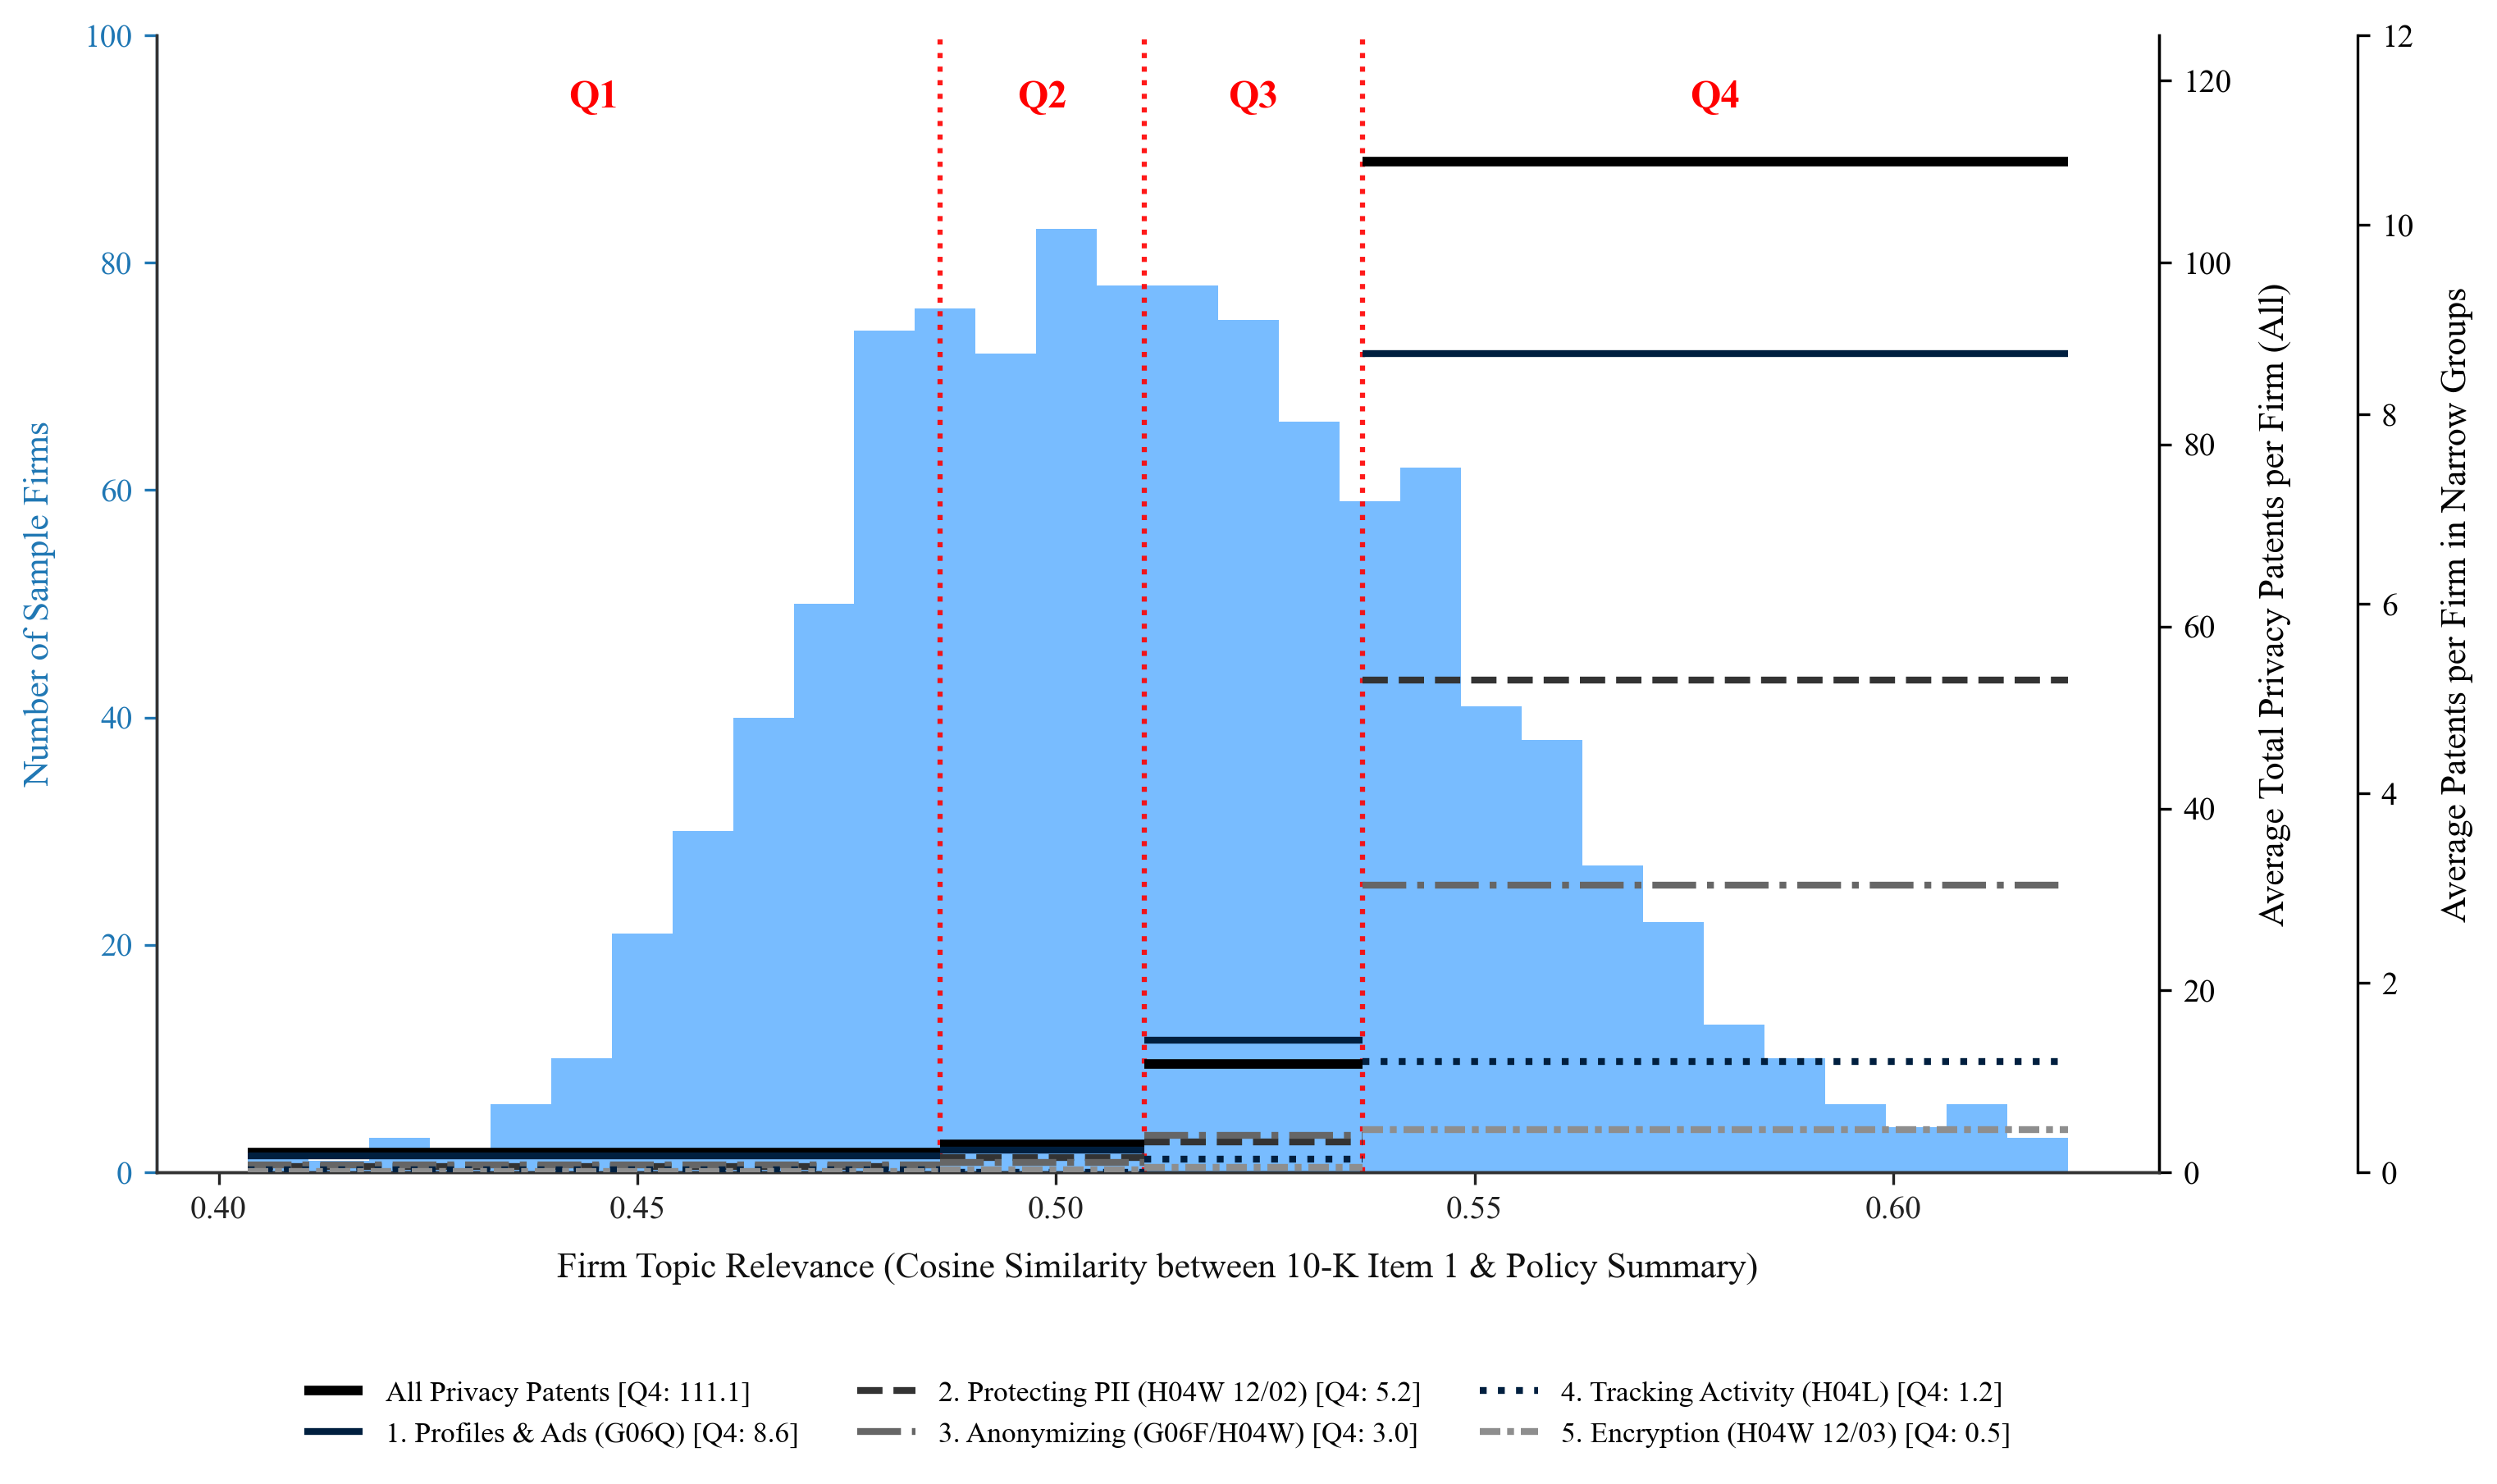
\includegraphics[width=\textwidth]{figures/fig_app_c_panel_a_topic_relevance.png}
    \end{minipage}\hfill
    \begin{minipage}{0.32\textwidth}
        \centering
        \textbf{\scriptsize Panel B: Pre/Post 2016 by Quartile}\par\vspace{2pt}
        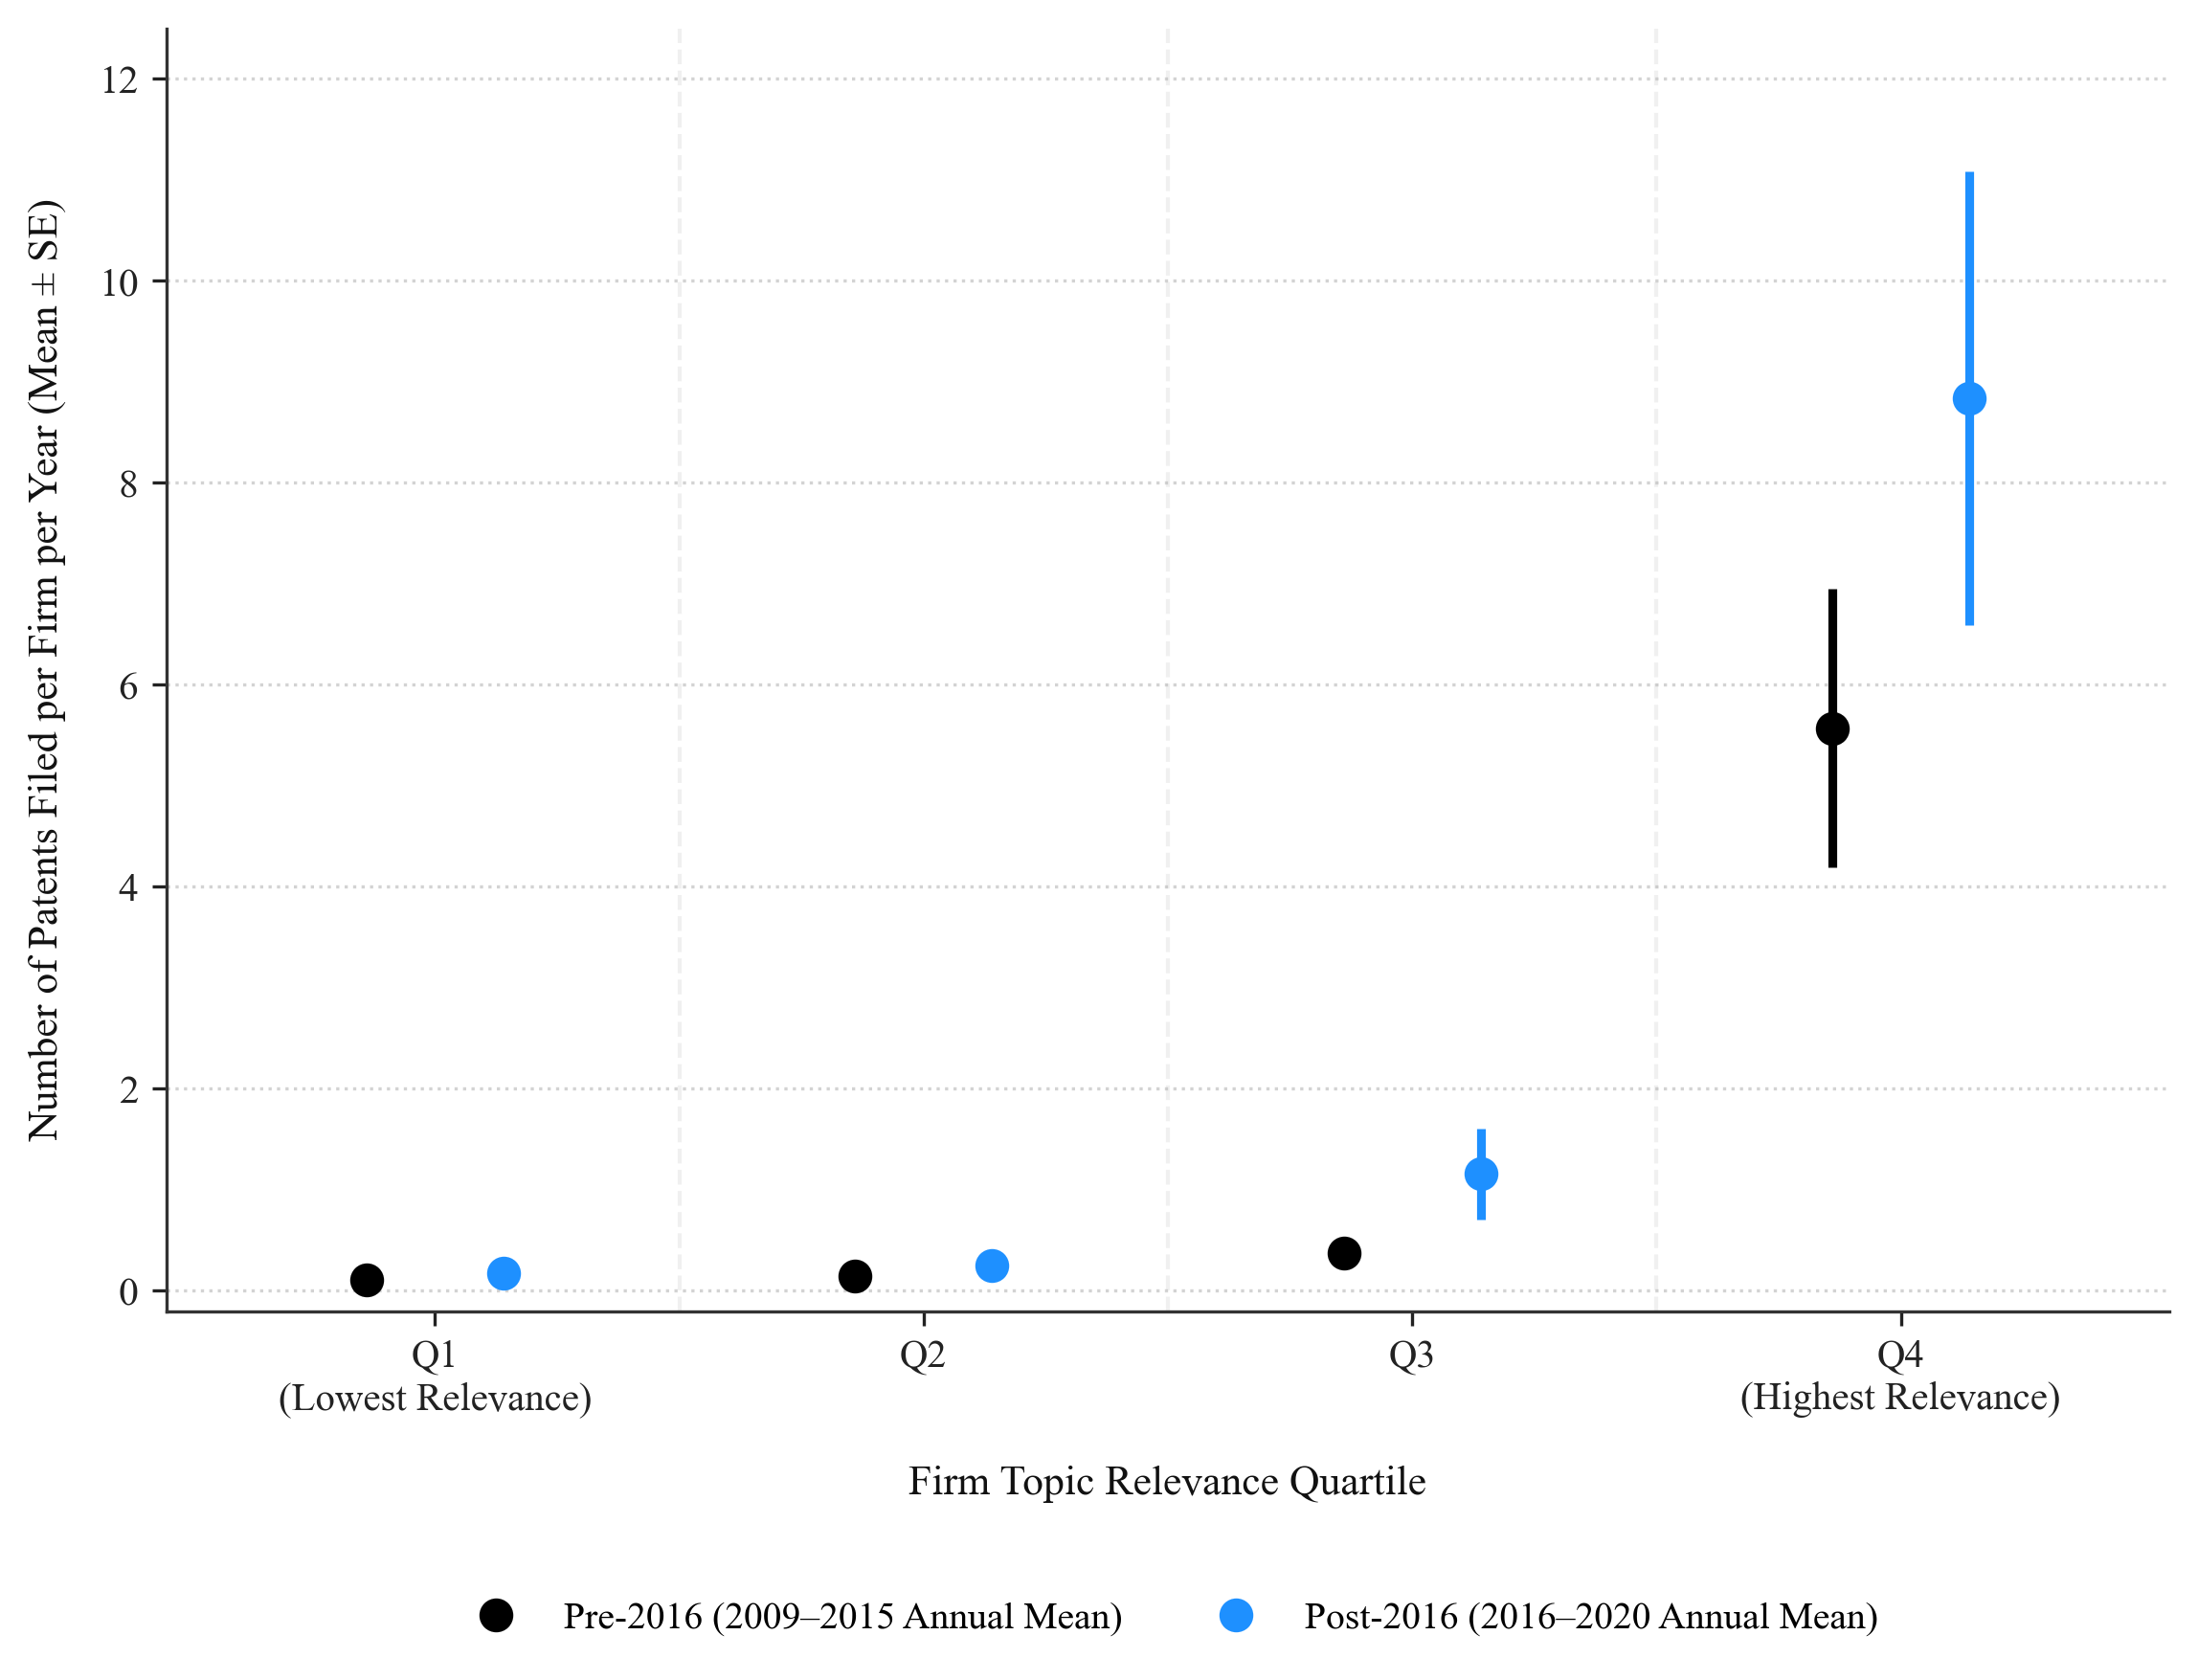
\includegraphics[width=\textwidth]{figures/fig_app_c_panel_b_quartiles.png}
    \end{minipage}\hfill
    \begin{minipage}{0.32\textwidth}
        \centering
        \textbf{\scriptsize Panel C: Pre/Post by Subclass}\par\vspace{2pt}
        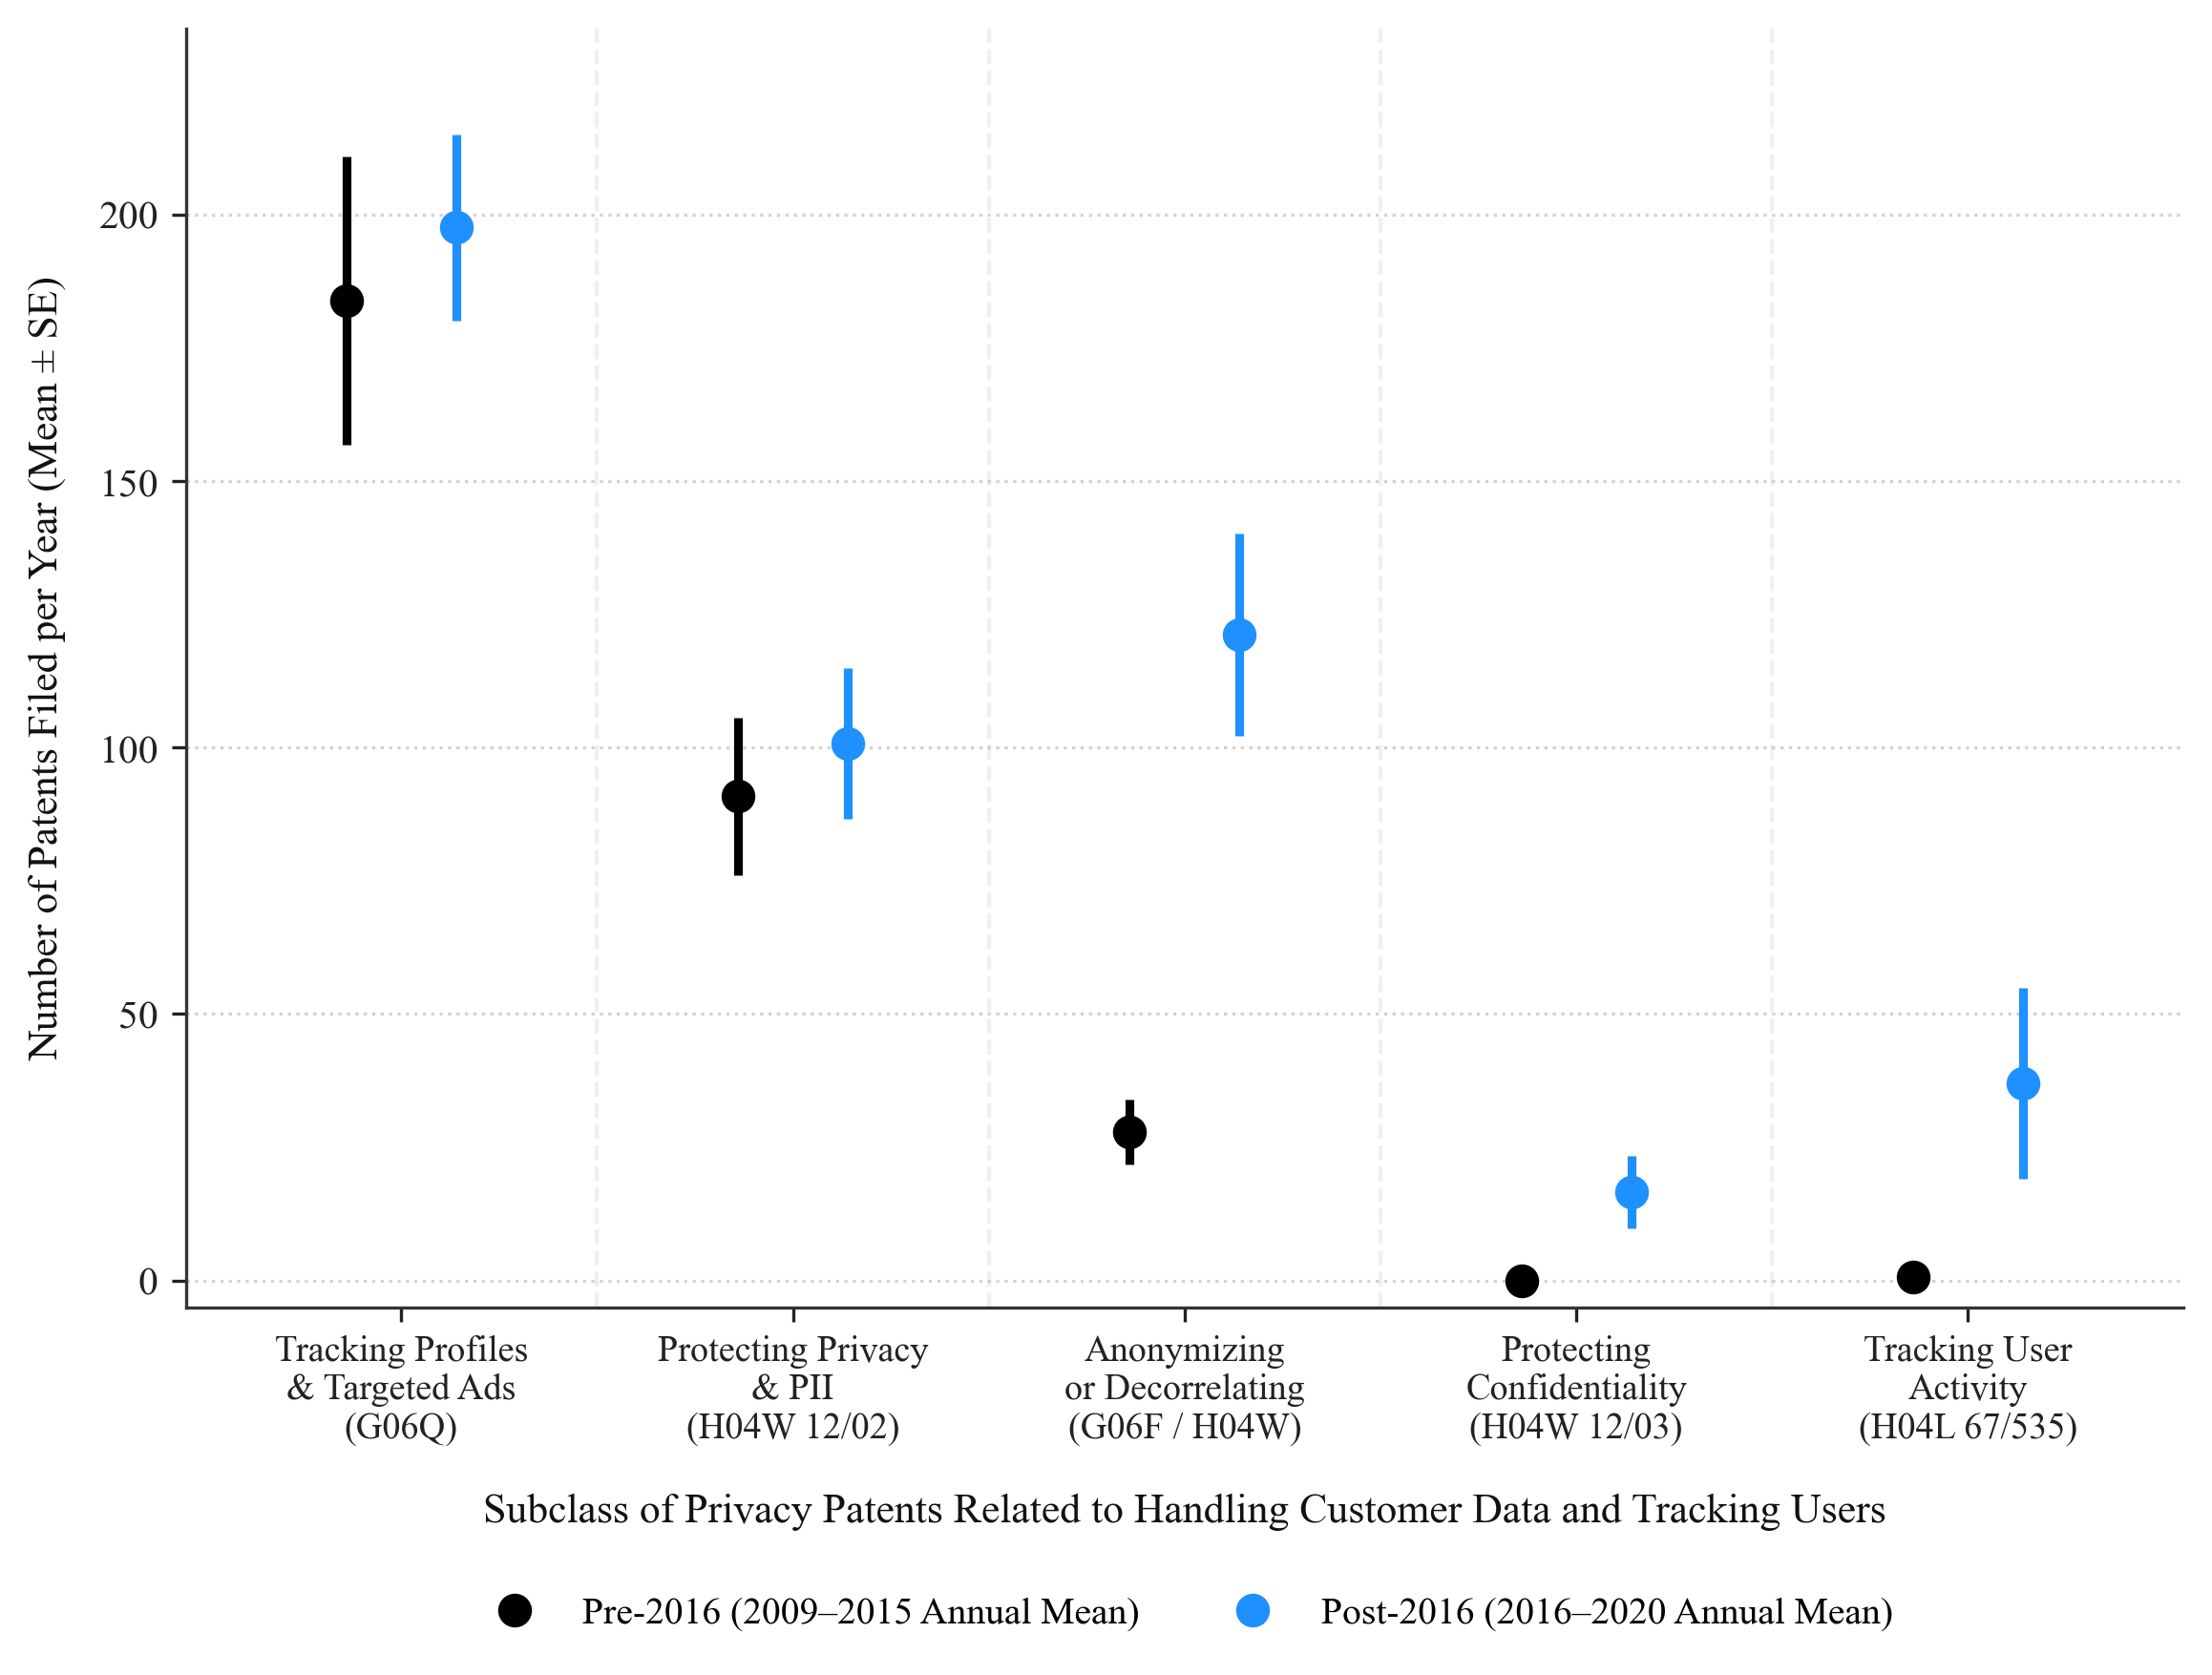
\includegraphics[width=\textwidth]{figures/fig_app_c_panel_c_subclasses.png}
    \end{minipage}
    \caption{\textbf{Topic Relevance and Privacy Patenting Responses Pre- and Post-2016.}}
    \vspace{4pt}
    {\footnotesize\textit{Notes: Sample comprises 1,058 publicly traded firms scored for policy relevance. Panel A shows patent intensity by relevance quartile. Panel B shows pre- vs. post-2016 changes by quartile. Panel C shows annual filing changes across privacy technology subclasses.}\par}
\end{figure}

To evaluate the dynamic trajectory of this response, Figure 5 (referred to as Figure 6 in the pipeline) presents annual event-study estimates of patenting probability from 2009 to 2020 relative to 2015 across topic relevance quartiles ($Q_1$ to $Q_4$). The outcome in each panel is an indicator equal to one if firm $i$ filed at least one patent application in year $t$ in the focal technology group, estimated using firm fixed effects with standard errors clustered at the firm level.

\begin{figure}[htbp]
    \centering
    \begin{minipage}{0.48\textwidth}
        \centering
        \textbf{\footnotesize Panel A: Anonymizing / Decorrelating Data}\par\vspace{2pt}
        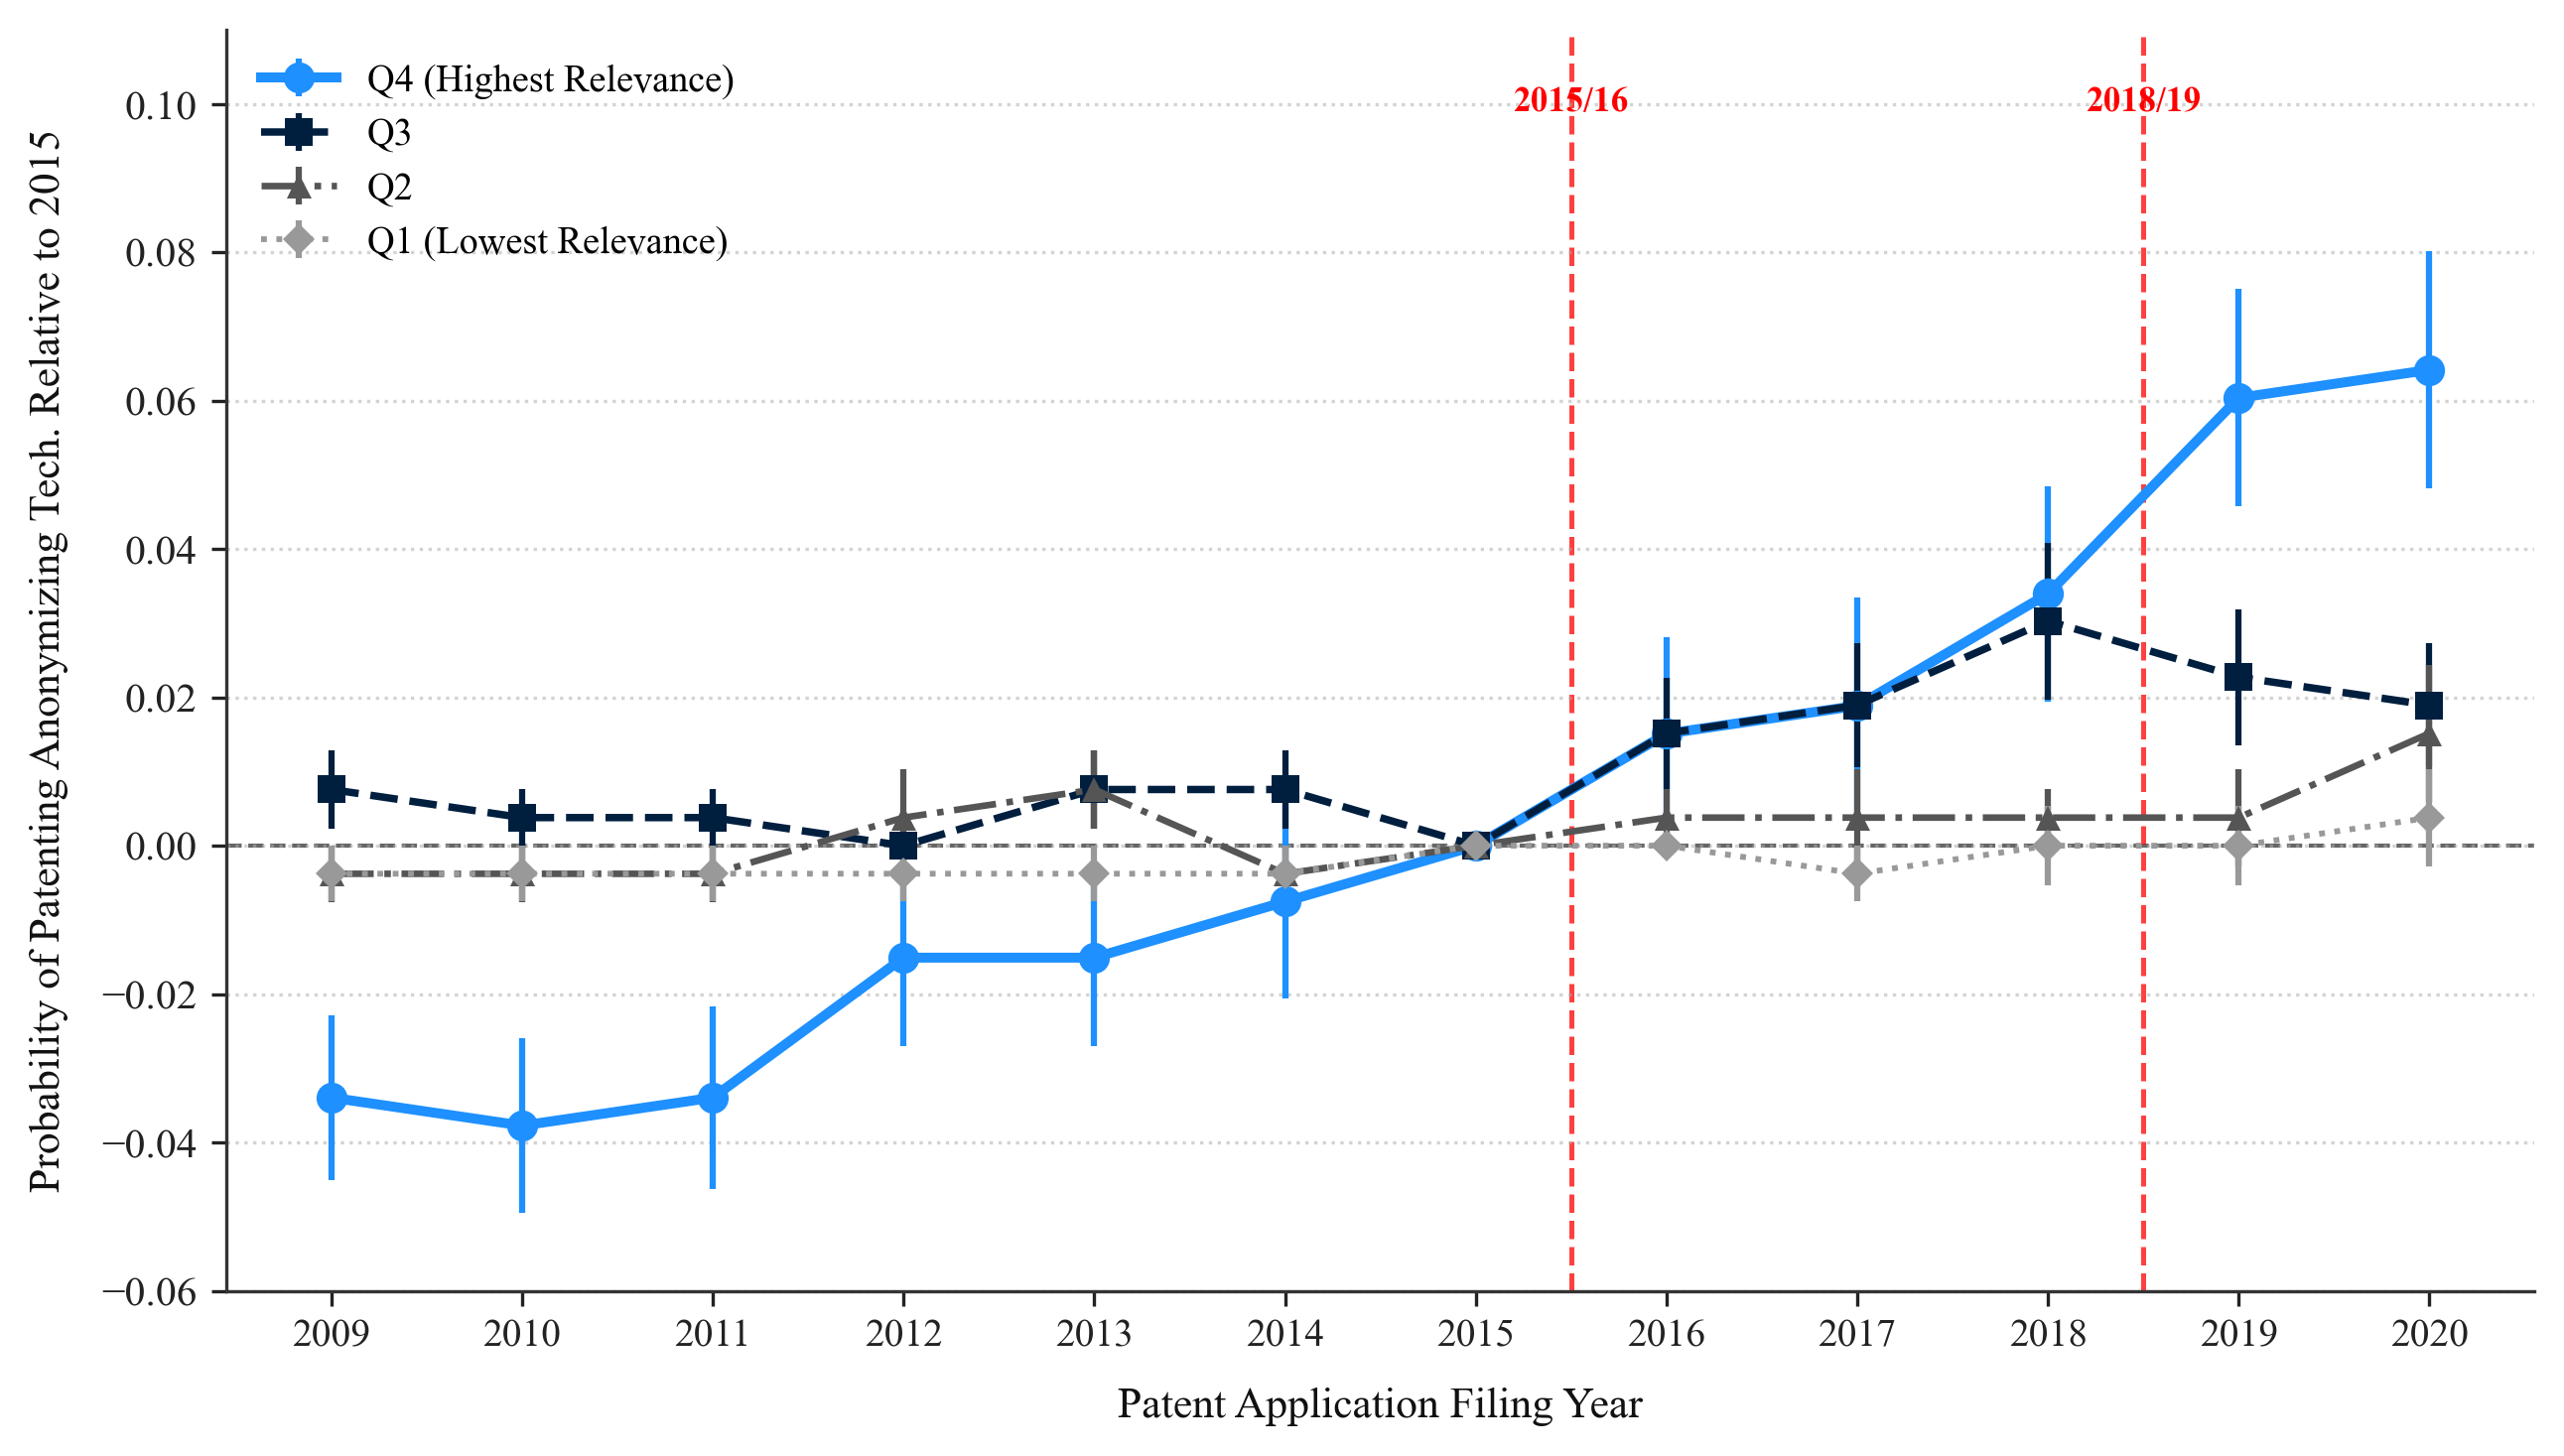
\includegraphics[width=\textwidth]{figures/fig_app_c_fig6_panel_a_anonymizing.png}
    \end{minipage}\hfill
    \begin{minipage}{0.48\textwidth}
        \centering
        \textbf{\footnotesize Panel B: Tracking User Activity}\par\vspace{2pt}
        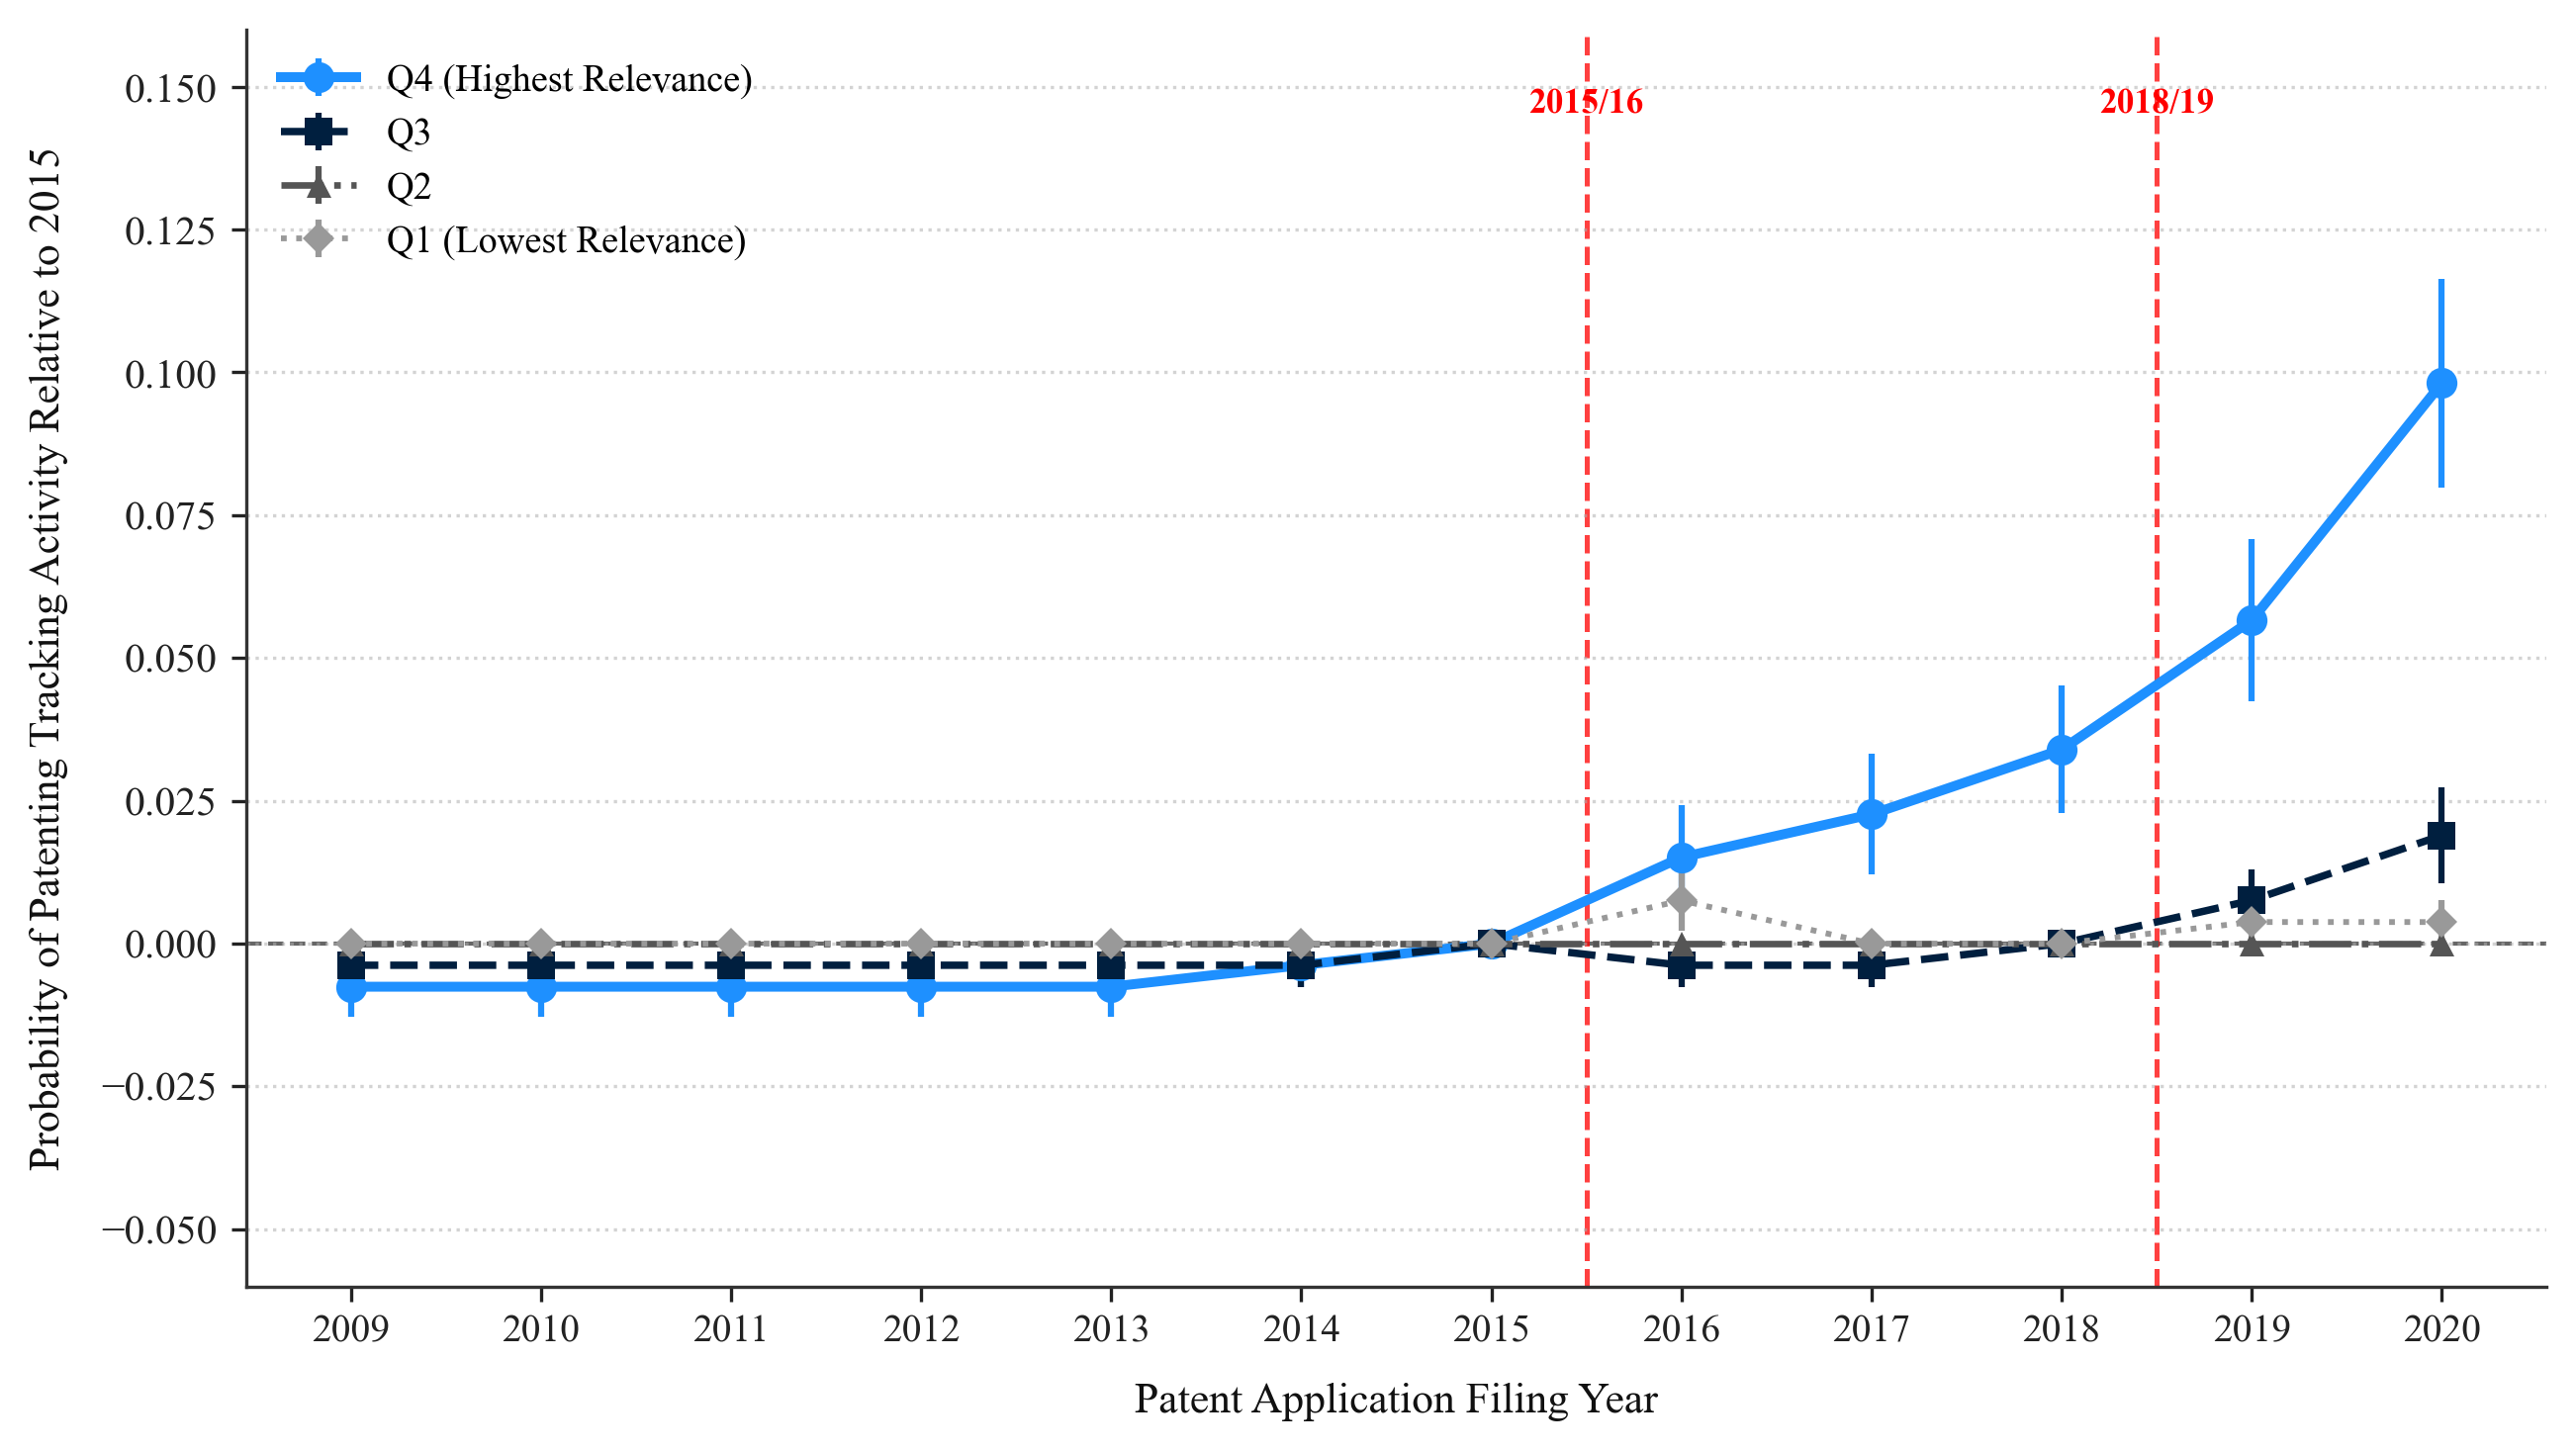
\includegraphics[width=\textwidth]{figures/fig_app_c_fig6_panel_b_tracking.png}
    \end{minipage}
    \caption{\textbf{Annual Event-Study Estimates of Patenting Probability Relative to 2015 by Relevance Quartile.}}
    \vspace{4pt}
    {\footnotesize\textit{Notes: Sample comprises 1,058 firms. Estimated using firm fixed effects with standard errors clustered at the firm level. Vertical capless error bars represent 95\% confidence intervals. Vertical red dashed lines indicate the 2015/2016 policy transition and the 2018/2019 GDPR/CCPA enforcement milestone. Panel A evaluates Anonymizing or Decorrelating Data (CPC G06F 21/6254, H04W 12/033); Quartile 4 firms exhibit a sharp increase of $+6.0$ pp in 2019 ($p < 0.001$) and $+6.4$ pp in 2020 ($p < 0.001$). Panel B evaluates Tracking User Activity (CPC H04L 67/535); Quartile 4 firms experience a continuous rise up to $+9.8$ pp in 2020 ($p < 0.001$). Pre-trends are flat across all quartiles.}\par}
\end{figure}

In summary, this empirical exercise demonstrates how our AI-enabled pipeline constructs auditable, highly predictive firm-level measures that make it possible to study organizational innovation responses to policy debates.

\newpage
\section*{Appendix D. Reproducible and Adaptable Data Pipelines with Coding Agents}
\addcontentsline{toc}{section}{Appendix D. Reproducible and Adaptable Data Pipelines with Coding Agents}

While this data pipeline leverages AI tools to perform critical measurement tasks, an additional structural benefit is emerging: research pipelines shared via online repositories (like GitHub) in machine-readable formats can be rapidly deployed, verified, and adapted by autonomous coding agents.

Rather than treating papers as static documents, online repositories serve as active software environments where researchers share modular tools. To demonstrate this capability, the accompanying repository folder (\href{https://github.com/HC-Geopolitics-Innovation/LLM-Text-Analysis-and-Synthesis/tree/main/X2%20-%20Example%20of%20Reproducing%20and%20Adapting%20the%20Research%20Pipeline}{\texttt{X2 - Example of Reproducing and Adapting the Research Pipeline/}}) provides:
\begin{enumerate}
    \item \textbf{Sample Agent Prompt:} An actionable prompt (\href{https://github.com/HC-Geopolitics-Innovation/LLM-Text-Analysis-and-Synthesis/blob/main/X2%20-%20Example%20of%20Reproducing%20and%20Adapting%20the%20Research%20Pipeline/X1%20-%20Sample%20Agent%20Prompt%20For%20Adapting%20Research%20Pipeline%20To%20New%20Question.md}{\texttt{X1 - Sample Agent Prompt For Adapting Research Pipeline To New Question.md}}) instructing an LLM coding agent to read the repository architecture, inspect input corpora, and adapt the staged methodology to a new research setting (e.g., regulatory debate surrounding renewable energy and corporate carbon emission innovation).
    \item \textbf{Implementation Plan:} A full, researcher-evaluable implementation plan (\href{https://github.com/HC-Geopolitics-Innovation/LLM-Text-Analysis-and-Synthesis/blob/main/X2%20-%20Example%20of%20Reproducing%20and%20Adapting%20the%20Research%20Pipeline/X2%20-%20Sample%20Implementation%20Plan%20Generated%20by%20Pipeline.md}{\texttt{X2 - Sample Implementation Plan Generated by Pipeline.md}}) detailing step-by-step adaptations, schema crosswalks (from CPC privacy codes to Y02 climate mitigation patent classifications), verification checkpoints, and execution timelines.
\end{enumerate}

Researchers can provide this prompt to their own AI tools, evaluate the proposed implementation plan, and deploy adaptable pipelines for organizational and social science research.

\end{document}
